
\chapter{轨道交通联锁软件可信评估工具研究}
\label{ch5}

\begin{kaishu}
	本章主要介绍轨道交通联锁软件可信评估工具的分析、设计和实现过程。章末以苏州轨道交通二号线的联锁软件产品为例,介绍工具的具体使用流程。
	
\end{kaishu}

\section{系统分析与设计}
本节首先对系统进行分析,用例图可以明确系统的用户及其对应的功能。接着系统结构图列出了系统的主要模块,最后流程图详细描述了业务流程。

\subsection{系统分析}
由于现在各界人士对软件可信性的关注度越来越高,在可信领域也有很多可信评估工具的出现,通过调研,发现一些工具在以下几个方面仍存在不足:
\begin{itemize}
    \item 评估工具只针对某个特定的软件;
    \item 评估工具与用户交互的界面设计复杂,实际操作繁琐,使用者难以上手;
    % \item 评估工具用户界面不友好,操作繁琐,给用户带来负担;
    \item 评估工具仅关注当前评估的软件可信性,而没有给出相应的改进建议或者指导。
\end{itemize}

开发工具的目的是让程序代替人类执行某些操作,减轻人们工作负担的同时高效地提供准确的结果。本文在之前的评估工具的基础上,主要在以下几个方面做了优化:
\begin{itemize}
    \item 评估工具对轨道交通领域的所有联锁软件均适用,仅需要自定义评估可信评估数据表即可;
    \item 评估过程最大程度实现自动化,尽可能减少用户的操作;
    \item 评估结果展示当前评估软件产品的可信值与可信等级,同时对软件可信等级的提高,具体应如何改进,提供建议。
\end{itemize}

UML(Unified Modeling Language)
是针对采用面向对象开发系统的产品进行说明、可视化展示和撰写文档的一种标准建模语言,
%是一种统一建模语言,是为面向对象开发系统的产品进行说明、可视化和编制文档的一种标准语言,
是需求分析常用工具之一\cite{Li2017Research}。
其中用例图主要回答了两个问题:1、谁使用软件工具;2、工具的功能。从使用者的角度描述了系统工具的功能模块,并指出了各个功能的执行者。

本文设计的软件可信评估工具主要分为软件产品信息管理、全生命周期可信评估、评估结果三大模块。工具的使用人员包括项目负责人(管理员)和普通用户。软件产品信息管理模块包括软件产品信息维护和软件产品人员信息维护两个子模块;全生命周期可信评估即需求阶段可信评估、设计阶段可信评估、编码阶段可信评估和测试阶段可信评估,每个阶段可信评估有可信证据输入、权重分配和可信值计算三个功能点;评估结果包含了数据可视化和生成评估报告子模块,主要用于数据展示和提供改进意见。系统的用例图见图\ref{fig:5_01}:
\begin{figure}[H]
	\centering
	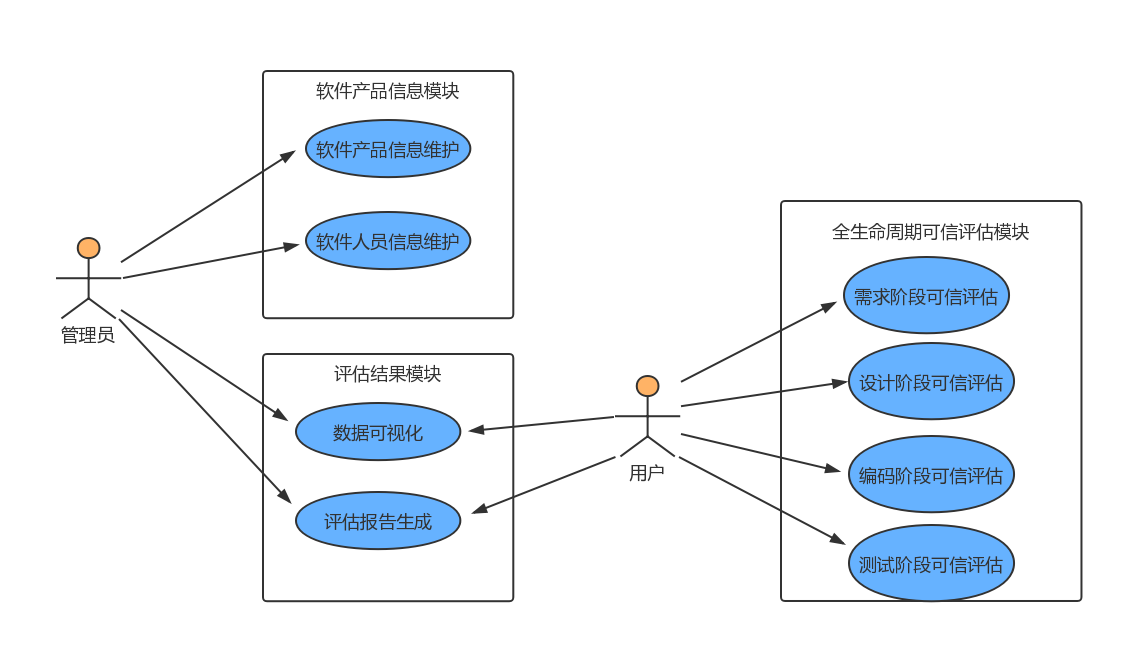
\includegraphics[width=15cm,height=10cm]{fig/5_01.png}
	\caption{联锁软件可信评估工具用例图}
	\label{fig:5_01}
\end{figure}



\subsection{系统设计}
工具共包含三大模块:基本信息管理模块、全生命周期可信评估模块和评估结果输出模块。基本信息模块由软件产品信息维护和相关人员信息维护组成。其中全生命周期可信评估模块分为需求、设计、编码和测试四个阶段可信评估子模块,每个子模块有可信证据输入、权重分配和可信值计算三个功能;评估结果输出模块包括数据可视化和评估报告生成,数据可视化子模块主要是图表分析,评估报告生成子模块给出软件的可信等级以及改进意见。图\ref{fig:5_03_0}是系统结构图。

\begin{figure}[htb]
	\centering
	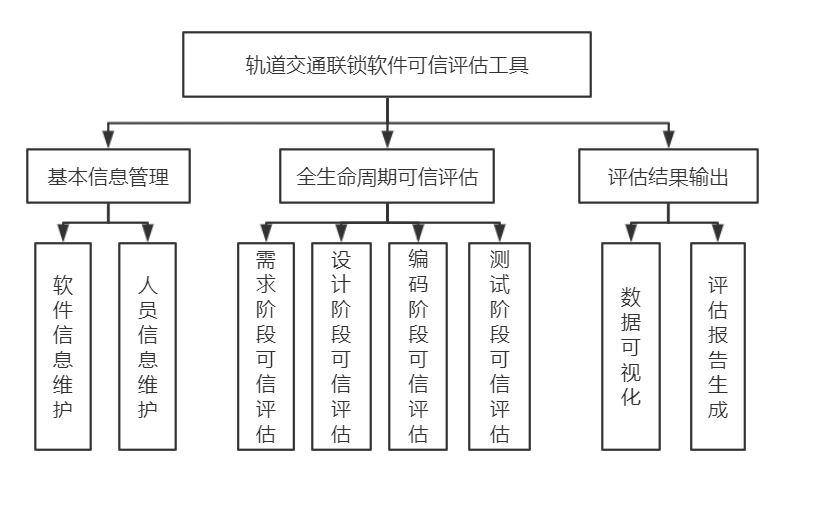
\includegraphics[width=13cm]{fig/5_03_0.png}
	\caption{联锁软件可信评估工具系统结构图}
	\label{fig:5_03_0}
\end{figure}

整个系统的业务流程是:首先录入待评测的轨道交通联锁软件产品相关信息后,从需求阶段开始进行全生命周期的可信评估,四个阶段评估完成之后对数据进行可视化展示,显示每个阶段属性和子属性可信值图谱和双柱形图,并生成评估报告,给出当前评估软件的可信等级并对之后的开发过程提出建议。流程图如\ref{fig:5_02}。

\begin{figure}[htb]
	\centering
	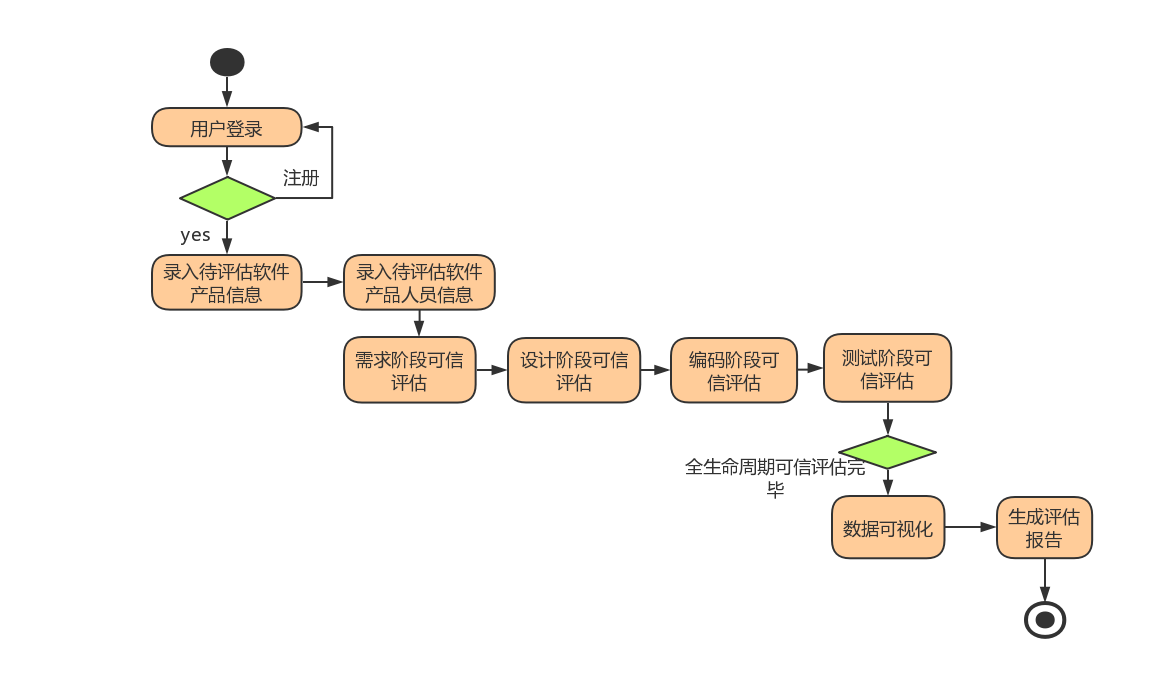
\includegraphics[width=15cm,height=10cm]{fig/5_02.png}
	\caption{联锁软件可信评估工具活动图}
	\label{fig:5_02}
\end{figure}


\section{轨道交通联锁软件评估工具实现}
轨道交通联锁软件评估工具实现整体采用模型-视图-控制器模式,简称MVC(Model View Controller)模式。用一种将业务逻辑、数据模型和UI界面显示分离开来的方式编写代码,将软件系统分为了三个部分:模型负责存储系统的中心数据,即实体类;视图负责用户交互;控制器处理用户输入的信息,负责从视图读取数据,并向模型发送数据。\cite{mvc体系结构}下图表示了这三者之间的关系\ref{fig:5_03}。工具后台采用当下流行的springboot技术,可以简化开发过程,省去很多繁冗的XML文件配置。工具模板引擎选择和springboot配套的thymeleaf,渲染数据到前端页面。数据库同时使用了MySQL和MongoDB。MySQL是一种关系型数据库,用来存储软件产品信息和软件产品人员信息,对MySQL的操作通过ibatis框架配置的映射文件。MongoDB是当下用的比较多最接近关系型数据库的非关系数据库,用来存储可信证据表,文档内部采用键值形式保存数据。工具主页如图\ref{fig:5_03_1}所示。
\begin{figure}[H]
	\centering
	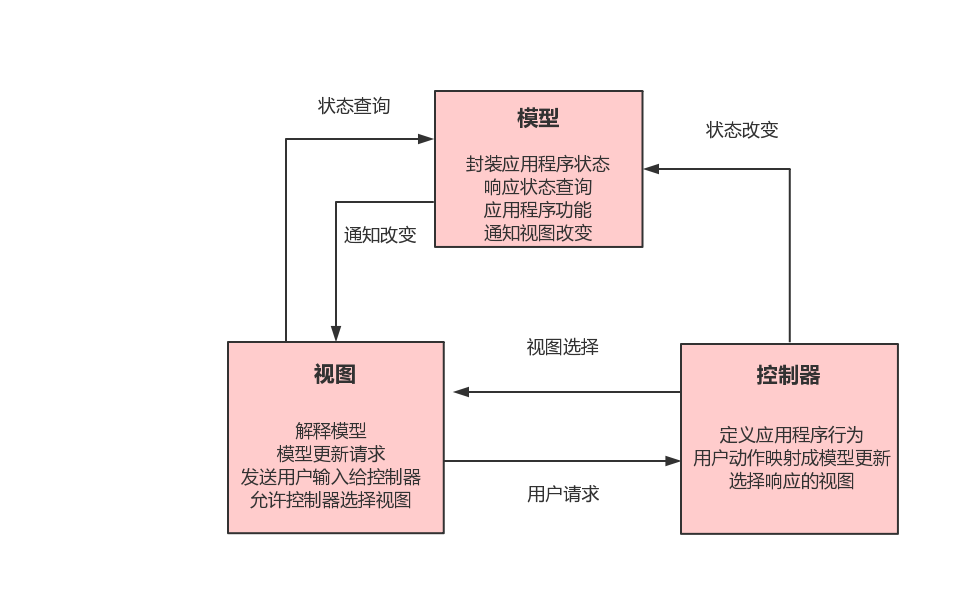
\includegraphics[width=13cm]{fig/5_03.png}
	\caption{MVC模式体系结构图}
	\label{fig:5_03}
\end{figure}

\begin{figure}[H]
	\centering
	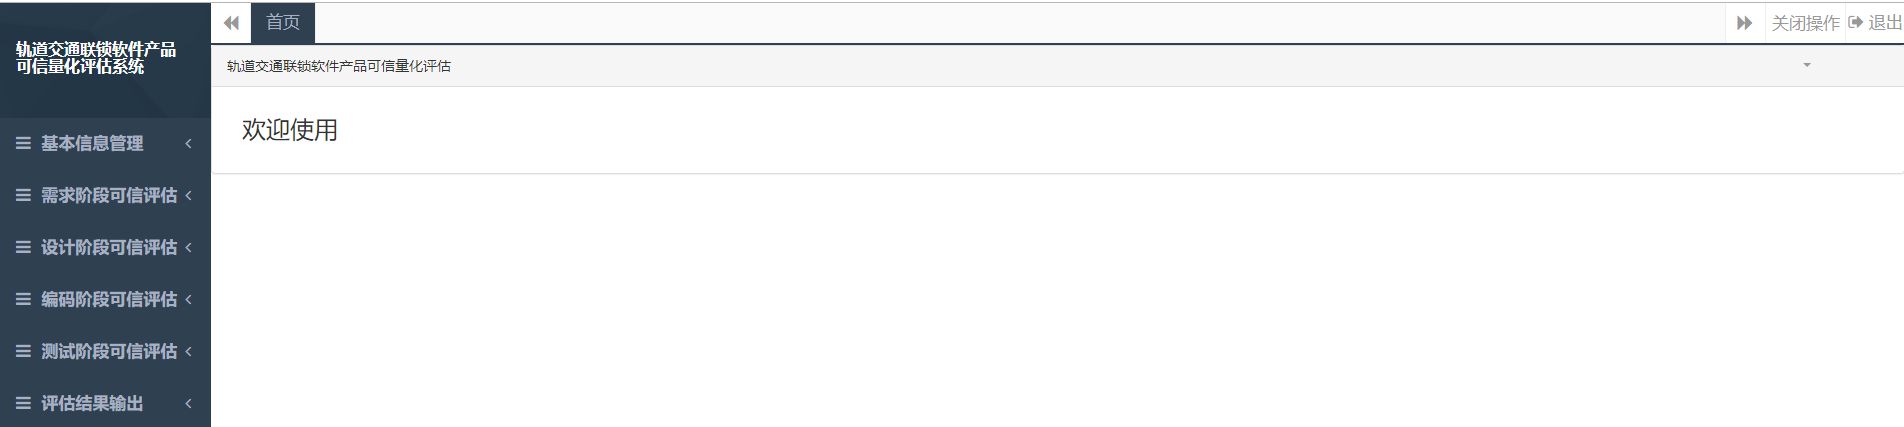
\includegraphics[width=13cm]{fig/5_03_1.png}
	\caption{工具主页}
	\label{fig:5_03_1}
\end{figure}

\subsection{基本信息管理实现}

(1)软件产品信息维护子模块

本文研究的工具并不是针对某一个单独的软件产品,在某个轨道交通联锁软件评估结束之后,可以添加其他软件产品进行评估。在对软件全生命周期进行可信评估之前,首先录入待评估软件的基本信息如软件产品编号,软件产品名称,软件产品状态(待评测、评测结束),项目组长,开发负责人等。可以有选择地对当前选中的软件产品信息进行删除或者修改。录入产品信息时候默认状态均为待评估,查看评估报告按钮不可用,评估过程完成之后,状态自动显示为评估结束,可点击查看按钮查看评估报告。界面如图所\ref{fig:5_04}示。

\begin{figure}[htb]
	\centering
	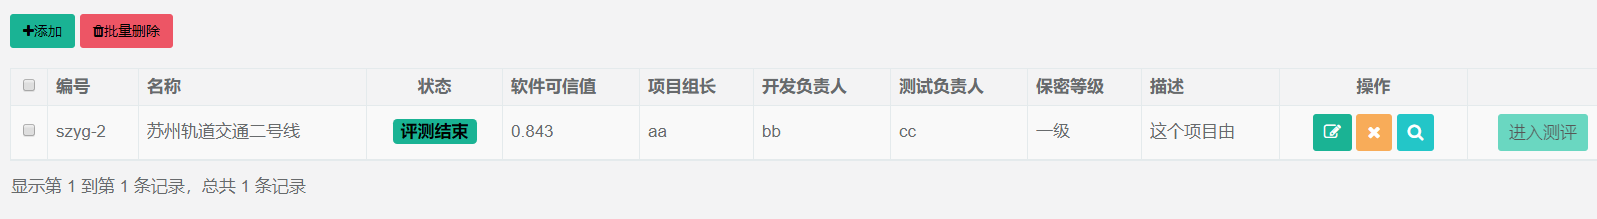
\includegraphics[width=14cm,height=3.5cm]{fig/5_04.png}
	\caption{软件产品信息维护界面}
	\label{fig:5_04}
\end{figure}


(2)软件人员信息维护子模块

对软件产品评估的同时也要录入负责整个软件产品开发过程的每个工作人员,若评估结果不是很理想,这样有利于决策人员之后制定改进计划,将分配分配到具体的负责人员。项目组的成员可能会变动,管理员可对人员信息进行维护,做增删改的操作,及时更新。

\begin{figure}[htb]
	\centering
	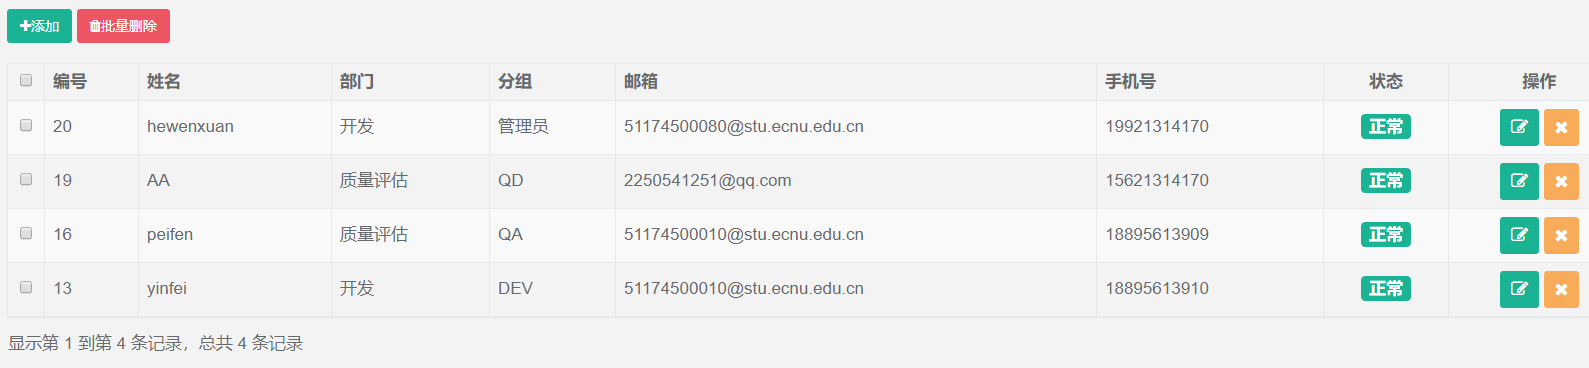
\includegraphics[width=13cm]{fig/5_05.png}
	\caption{软件人员信息维护界面}
	\label{fig:5_05}
\end{figure}

\subsection{全生命周期可信评估实现}

本文软件全生命周期可信评估包括需求、设计、编码和测试四个阶段的评估。四个阶段评估过程所涉及的方法类似,只是上传的可信证据表每个阶段不一样,所以本节仍围绕需求阶段可信评估展开叙述。

(1)可信证据输入

阶段可信评估首先上传可信证据(评估数据)表,表格部分内容如下。表格中每一行表示一条可信证据,从属性到度量元,每一个度量元对应一个度量指标,n和m的值均来源于软件产品开发过程依据的文档、程序等文件,保证真实有效。对于定量的度量元,m表示需要完成的指标数量,n表示未完成的指标数量;对于定量的度量元,直接由经验人士打分。

在界面最上方有个下载模板文件的按钮,上传的文件格式按照模板文件填写。填写Excel文件对用户来说操作比较简单,用户可以根据当前待评估的软件产品特点,自定义属性、子属性和度量元。Excel文件的数据填好保存之后,进入系统点击上传文件按钮,选择该阶段的可信证据表。若是上传失败,页面会弹出文件中数据不符合要求,返回修改数据格式即可。上传成功会将Excel中的数据显示在页面的表格中,点击左下角调整每页显示数据条数,点击分页条可进行翻页操作。用户也可在页面上对可信证据进行修改或批量删除。如果用户想添加表中没有的属性,必须相对应的添加子属性和度量元。UI界面如图\ref{fig:5_06}。

\begin{figure}[htb]
	\centering
	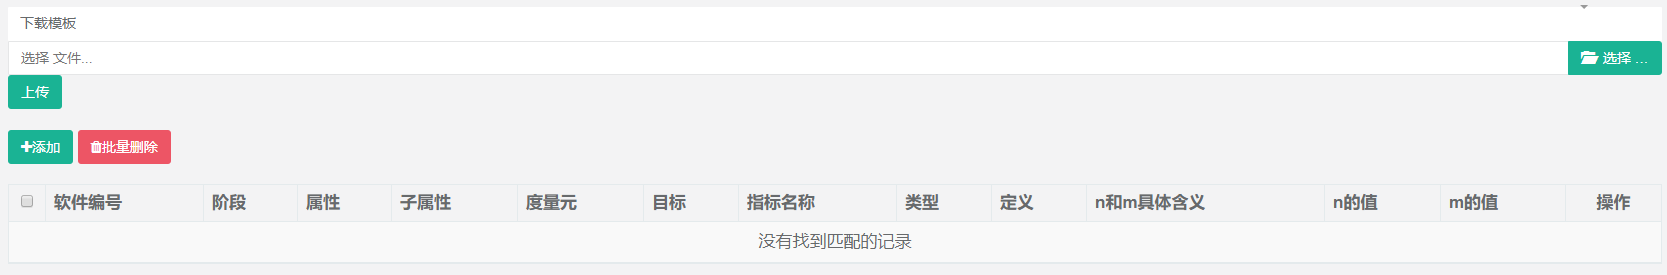
\includegraphics[width=13cm]{fig/5_06.png}
	\caption{需求阶段可信证据上传界面}
	\label{fig:5_06}
\end{figure}

% \begin{figure}[htb]
% 	\centering
% 	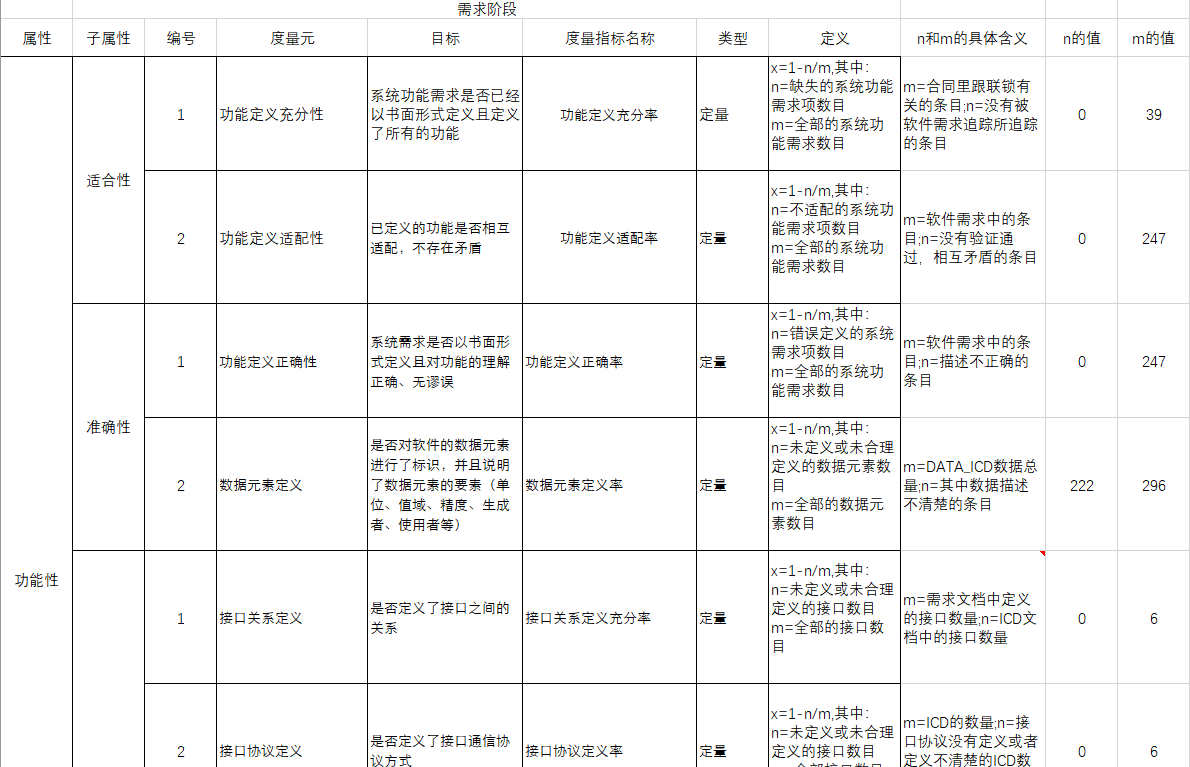
\includegraphics[width=13cm]{fig/5_6.png}
% 	\caption{需求阶段可信证据表详情}
% 	\label{fig:5_6}
% \end{figure}


(2)权重分配

阶段可信评估的第二步就是依次对属性、子属性和度量元进行权重分配。文献\cite{刘秋艳2017多要素评价中指标权重的确定方法评述}提到常见的赋权法主要有主观赋权法、客观赋权法和主客观结合赋权法,主观赋权法也称专家赋权,是一种比较成熟的方法,原始数据综合专家或者决策者根据经验主观判断给出的信息,将各指标元素依据主观上的重要程度进行比较、分配权重或计算得出其权重,
%其认为权重的实质是评价指标对于评价目标相对重要程度的量化体现。
这种方法考虑到客观存在的实际情况,从而使指标的权重更有现实意义。
%其中指标权重大小的排序基本与评价对象的实际情况相符合。
层次分析法就属于其中一种,是一种灵活而又实用的层次权重决策分析方法,适用于具有分层交错评价指标的目标系统,而目标值又难以定量描述的决策问题,同时对于样本数据量要求不高。
%层次分析法就属于其中一种,其使用范围很广,特别使用于缺乏样本数据且评价目标结构复杂以及领域专家对指标相对重要性大小程度有较为清晰认识的指标数量适中的评价体系。

由于实际应用中,联锁软件结构方程模型所需要的数据收集是一个漫长的过程,需要长时间的积累,因此,本节以确定属性权重为例,叙述层次分析法确定元素权重的过程。

\begin{itemize}
    
\item [1)] 建立阶段可信评估的层次结构模型

由上至下通常分为目标层、准则层、方案层。评估阶段可信值的层次结构模型如图\ref{fig:5_7}。
\begin{figure}[htb]
	\centering
	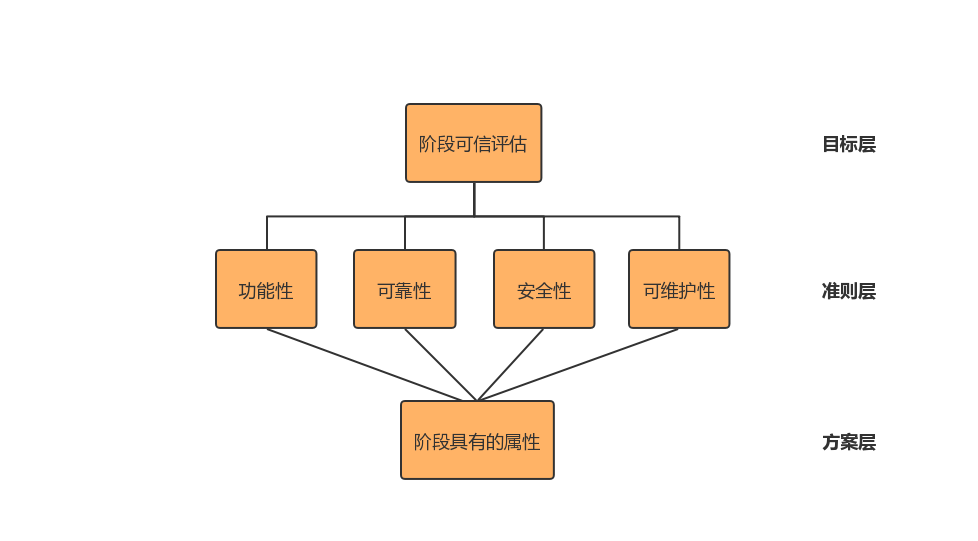
\includegraphics[width=13cm]{fig/5_12.png}
	\caption{阶段可信评估层次结构模型}
	\label{fig:5_7}
\end{figure}

\item [2)] 构造属性的正互反判断矩阵

准则层有四个属性,需要比较它们对目标层的影响程度,进而确定每个属性在该层所占的比重。属性之间两两进行比较,尺度选择1$-$9。构造正互反判断矩阵A,在矩阵中用$a_{ij}$表示第i个属性相对于第j个属性的重要程度,数值越大,表示越重要。
\[
A=(a_{ij})_{n*n}\begin{bmatrix}
a_{11} & a_{12} & \cdots & a_{1n}\\
a_{21} & a_{22} & \cdots & a_{2n}\\
\cdots & \cdots & \cdots & \cdots\\
a_{n1} & a_{n2} & \cdots & a_{nn}
\end{bmatrix}
\]
正互反判断矩阵满足一下性质:
\begin{itemize}
    \item [*] $a_{ij}$>0;
    \item [*] $a_{ij}=\frac{1}{a_{ji}}$
    \item [*] $a_{ii}$=1
\end{itemize}

\item [3)] 计算单排序向量并进行一致性检验

层次单排序就是确定下层因素对上层某一目标影响程度的过程,常用权值表示影响程度\cite{刘畅2006我国火电企业投资决策影响因素评价方法及模型研究}。一致性指标$CI=\frac{\lambda-n}{n-1}$,其中n为A的对角线元素之和,也为A的特征根之和;$\lambda$为A的最大特征根。随机一致性指标RI数值如下图,一般认为随机一致性比率$CR=\frac{CI}{RI}<0.1$时,则认为A通过一致性检验。对A计算最大特征值及其对应的特征向量,若此时A满足一致性,则归一化之后的特征向量即为权向量。

%\begin{figure}[htb]
%	\centering
%	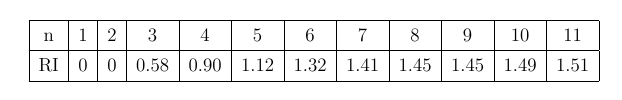
\includegraphics[width=13cm]{fig/5_07_1.png}
%	\caption{随机一致性指标RI数值}
%	\label{fig:5_07_1}
%\end{figure}

\begin{table}[!ht]
    \centering
    \caption{随机一致性指标RI数值}
    \begin{tabular}{|c|c|c|c|c|c|c|c|c|c|c|c|}
        \hline
         n & 1 & 2 & 3 & 4 & 5 & 6 & 7 & 8 & 9 & 10 & 11  \\
         \hline
         RI & 0 & 0 & 0.58 & 0.90 & 1.12 & 1.32 & 1.41 & 1.45 &1.45 &1.49 & 1.51\\
        \hline
    \end{tabular}
    \label{tab-5-1}
\end{table}
\end{itemize}

依次输入属性、子属性和度量元的正互反判断矩阵,计算属性相对阶段的重要程度、子属性占属性的权重、度量元占子属性的比重。在正互反矩阵输入界面底部,点击保存数据,可在下次加载页面的时候显示用户上次输入的数据回显,如果用户想要修改数据,只需修改变动的数据,不需要重新输入每个值,给用户带来方便。初始化时页面默认每个值都是1,如果用户在填写过程中想要清空所有值,点击重置数据即可。属性正互反矩阵输入页面点击下一步跳转到子属性正互反矩阵输入页面,再点击下一步是度量元正互反矩阵输入页面,三个正互反矩阵输入完成之后点击提交,如果一致性检验通过,会显示计算的属性,子属性,度量元的权重;否则页面会弹出某个正互反矩阵一致性检验没有通过的提示,返回修改数据。
\begin{figure}[htb]
	\centering
	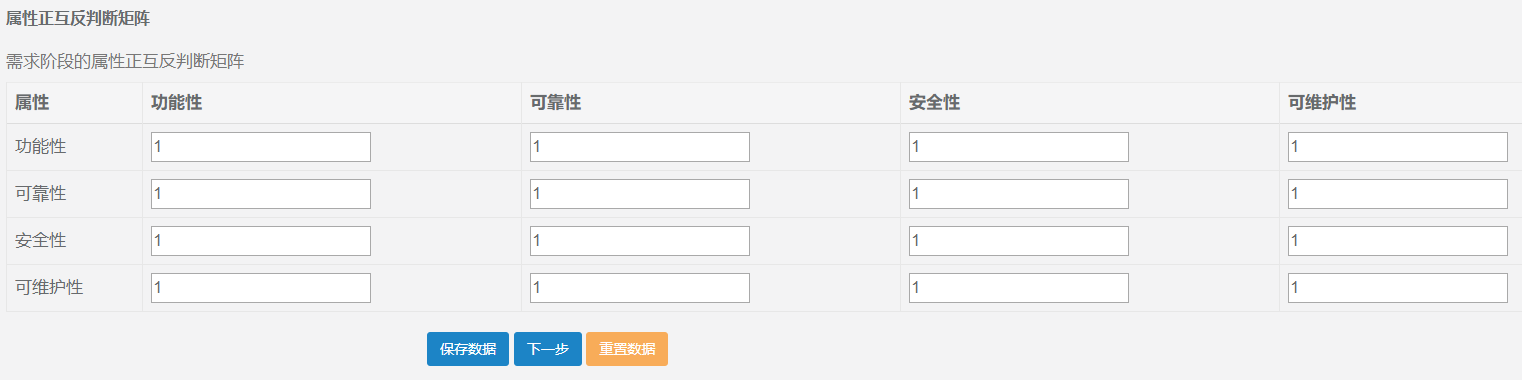
\includegraphics[width=13cm]{fig/5_07.png}
	\caption{需求阶段属性正互反矩阵输入界面}
	\label{fig:5_07}
\end{figure}


(3)可信值计算

点击左侧工具栏的可信值计算按钮,系统会将后台计算的可信值结果展示在页面上,可以很直观地表示属性和子属性的对应关系。定量度量元的可信值根据可信证据(评估数据)表中的n和m,通过公式$x=(1-\frac{n}{m})*10$计算;定性度量元则由专业人士打分,分值范围[0,10]。子属性的可信值根据下一层度量元的可信值和权重计算。属性的可信值根据其分解的子属性可信值和权重计算。阶段可信值由其包含的属性的可信值和权重得来。


% \begin{figure}[htb]
% 	\centering
% 	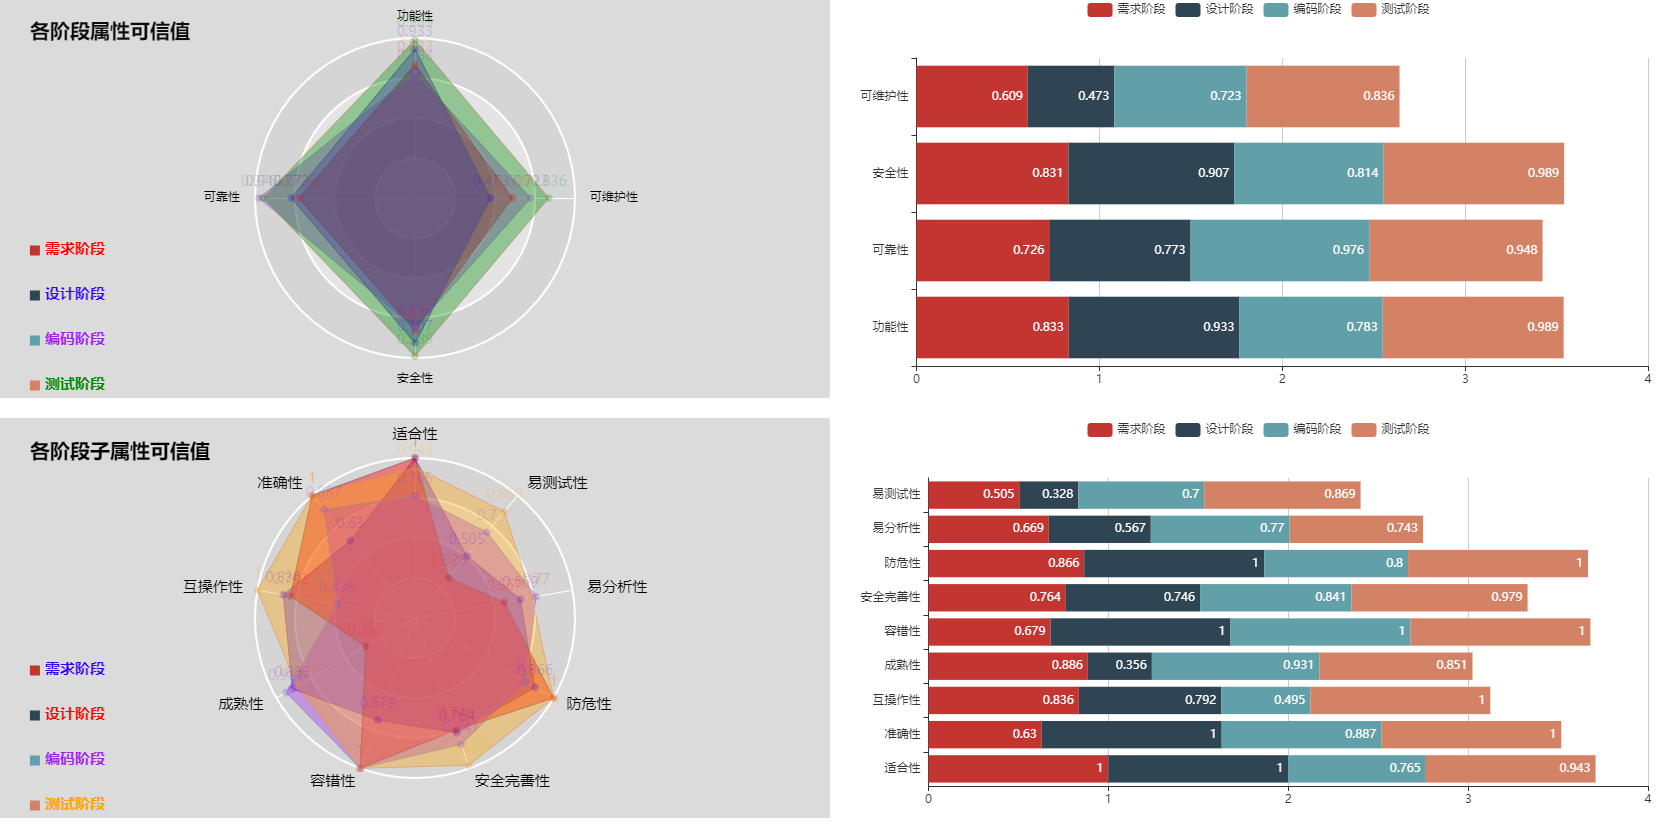
\includegraphics[width=13cm]{fig/5_08.png}
% 	\caption{需求阶段可信值计算界面}
% 	\label{5_08}
% \end{figure}


\subsection{评估结果输出实现}
这个模块是为了将轨道交通联锁软件评估的情况以可视化的形式向用户展示,用户可以可通过图表和报告看出当前软件产品存在的问题以及后续软件开发过程还需要在哪些方面进行改进。

(1)数据可视化

页面左侧是四个阶段属性和子属性的可信值图谱,右侧是四个阶段属性和子属性的堆叠条形图。通过可信值图谱,可以看出某个属性可信值在四个阶段比较,哪个阶段最小一目了然;还可以看出某个阶段所有属性可信值分布是否均匀。堆叠条形图具有更强的二维表现力,可以通过直条的长短清楚地看出具体可信值的大小,也可以清晰地比较某一维度数据的差异。
\begin{figure}[htb]
	\centering
	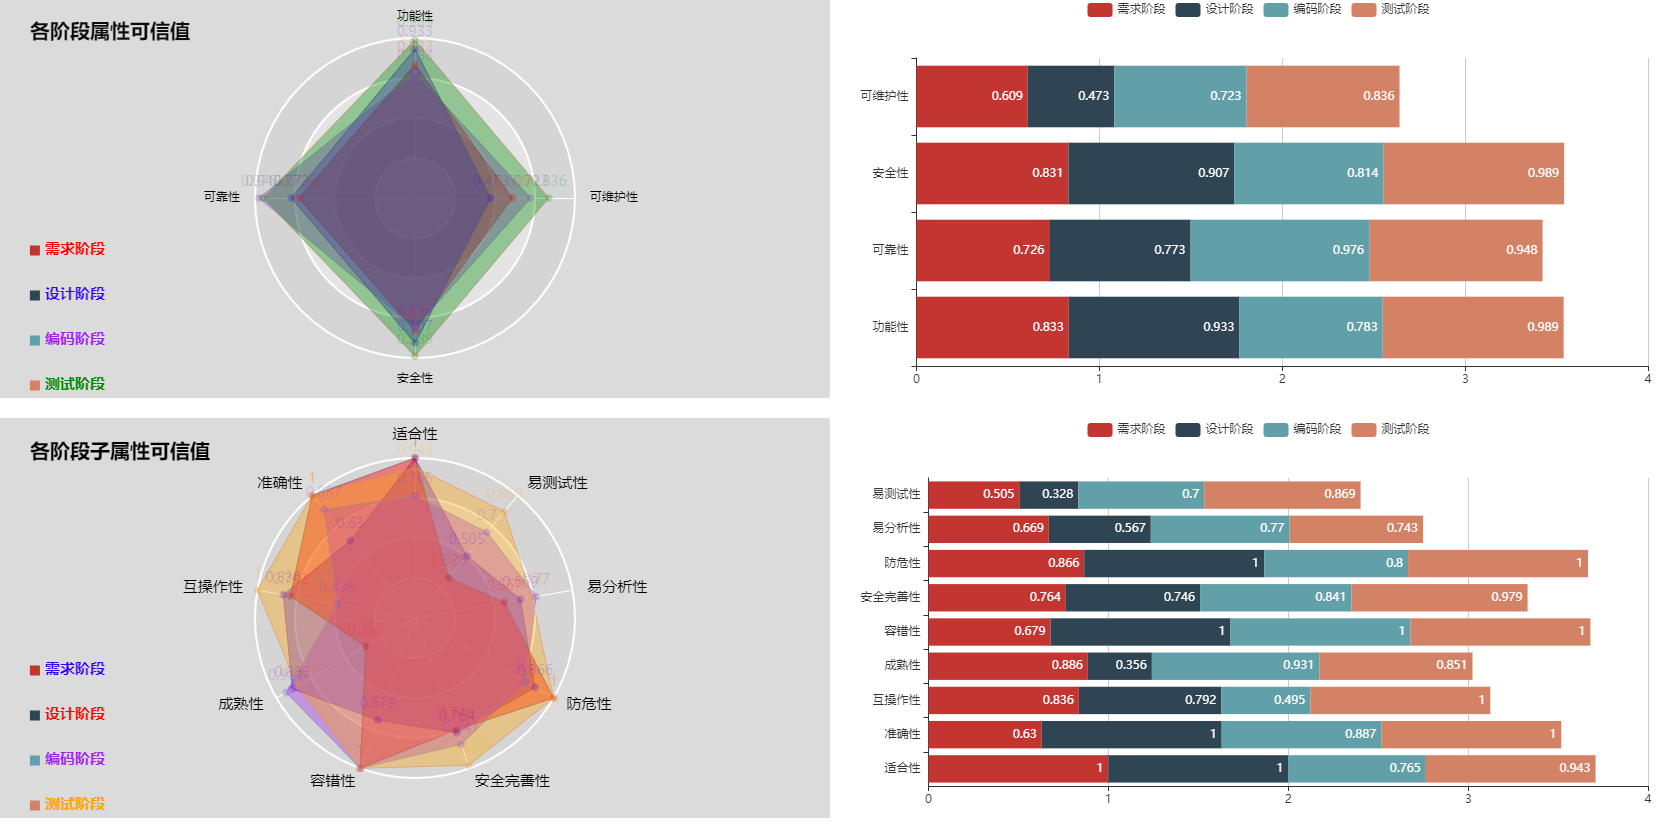
\includegraphics[width=13cm]{fig/5_08.png}
	\caption{四个阶段属性可信值图谱与堆叠条形图}
	\label{fig:5_08}
\end{figure}

图\ref{fig:5_09}具体地展示了每个阶段的所有信息,包括阶段可信值,属性可信值和权重,子属性可信值和权重,度量元可信值和权重。

\begin{figure}[htb]
	\centering
	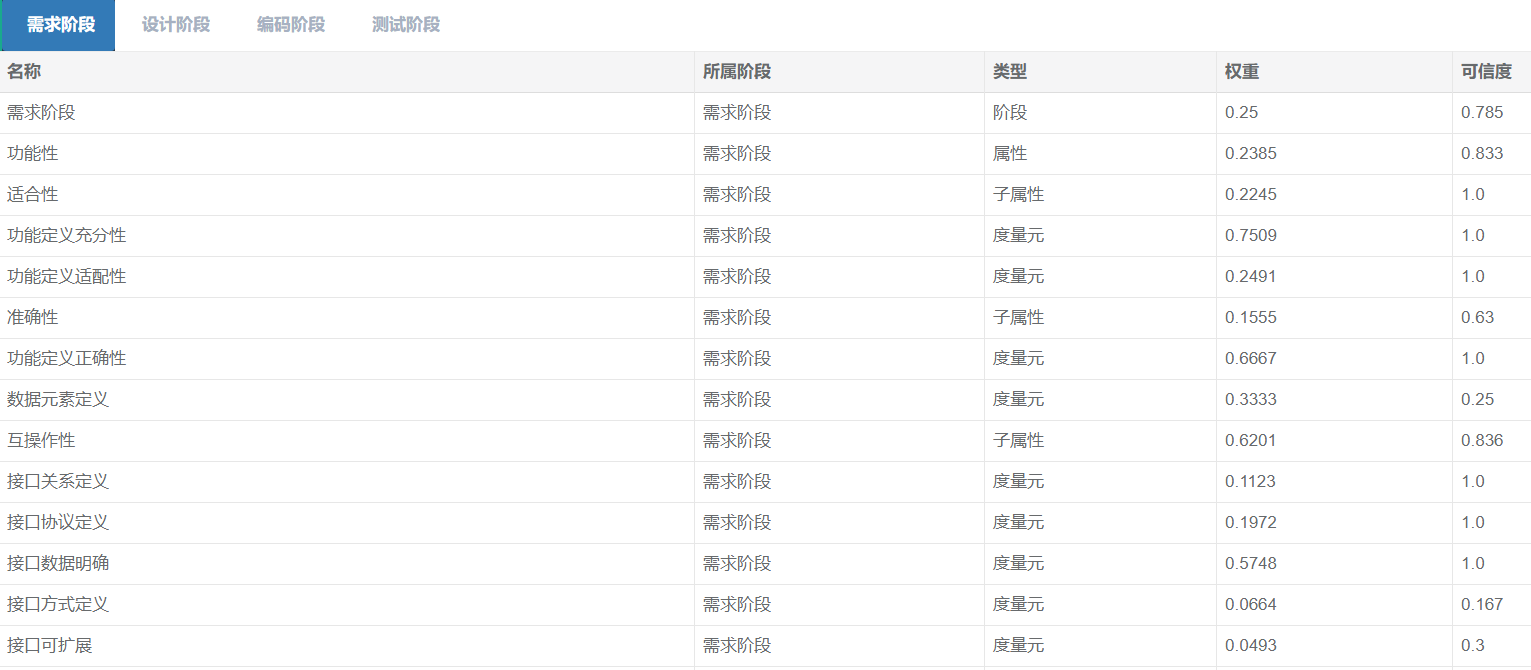
\includegraphics[width=13cm]{fig/5_09.png}
	\caption{四个阶段可信值表格界面}
	\label{fig:5_09}
\end{figure}

(2)评估报告生成

评估报告页面展示了待评估软件产品的名称、编号、可信值以及可信等级。
% 列出了软件全生命周期的属性的可信值和度量元的改进优先指数。
若当前软件可信等级小于等于三级,会相应地给出提高可信等级的改进建议。
\begin{figure}[htb]
	\centering
	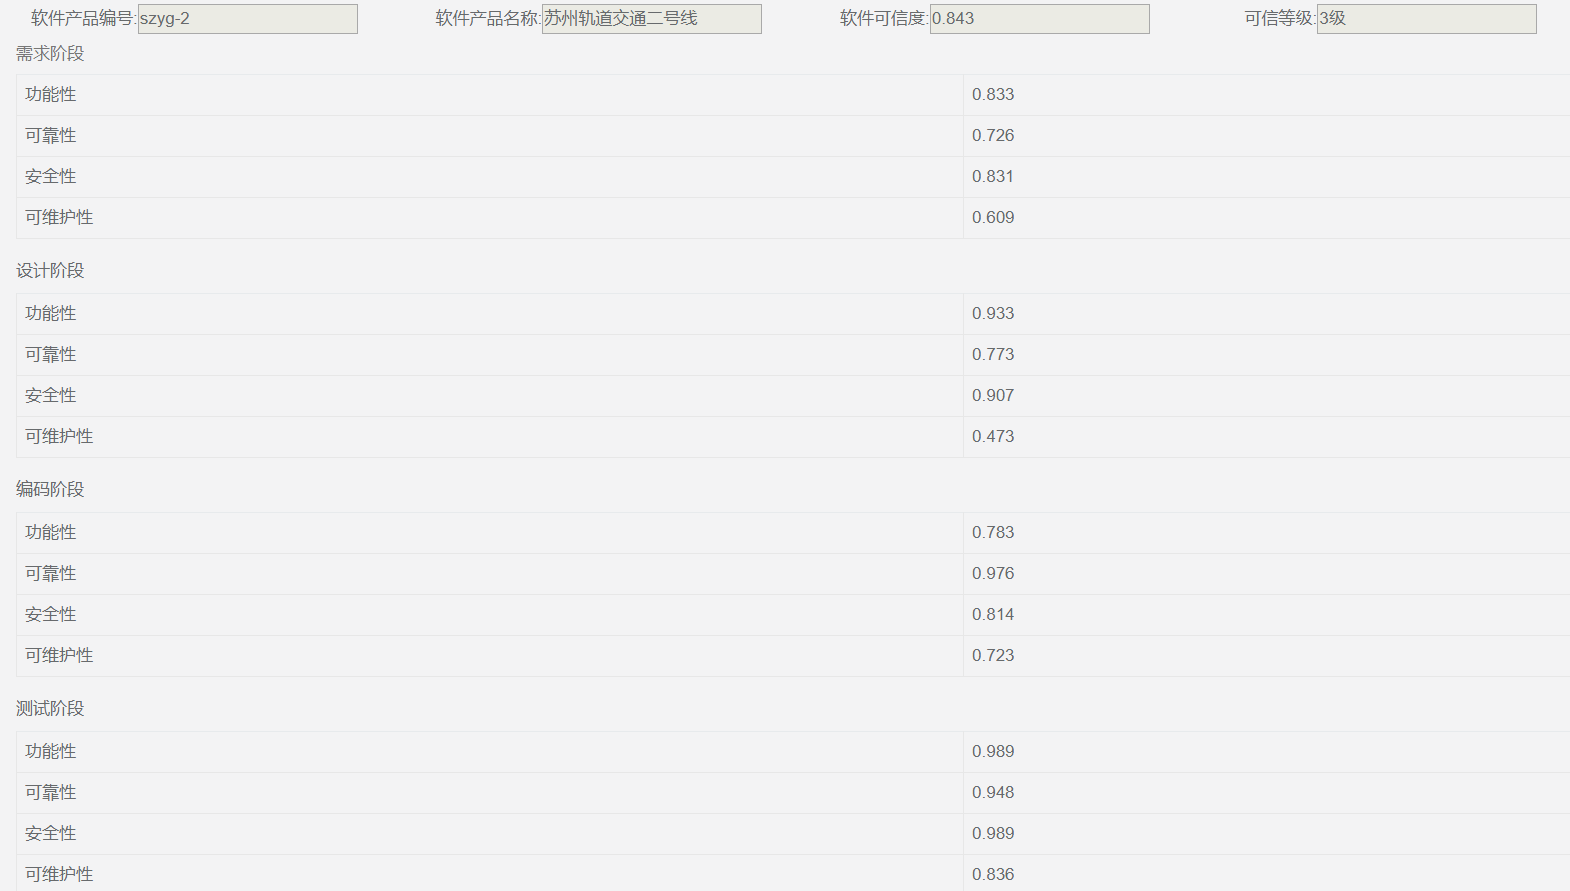
\includegraphics[width=13cm]{fig/5_10.png}
	\caption{评估报告界面}
	\label{fig:5_10}
\end{figure}

\section{轨道交通联锁软件评估工具使用}
本节以评估苏州有轨二号线联锁软件可信性为例,详细介绍工具使用流程。

浏览器中访问localhost:8081,轨道交通联锁软件可信测评工具的登录页面。已经注册过的用户可在表单中直接输入用户名和密码,校验通过即可使用工具,校验不通过如姓名或密码不对应,会提示错误信息。没有注册的用户点击注册链接,弹出用户注册页面,输入相应的信息,点击确定,则注册成功,跳转到登录界面,可用注册的用户名和密码进行登录。登录成功即进入首页,如图\ref{fig:5_11}
\begin{figure}[htb]
	\centering
	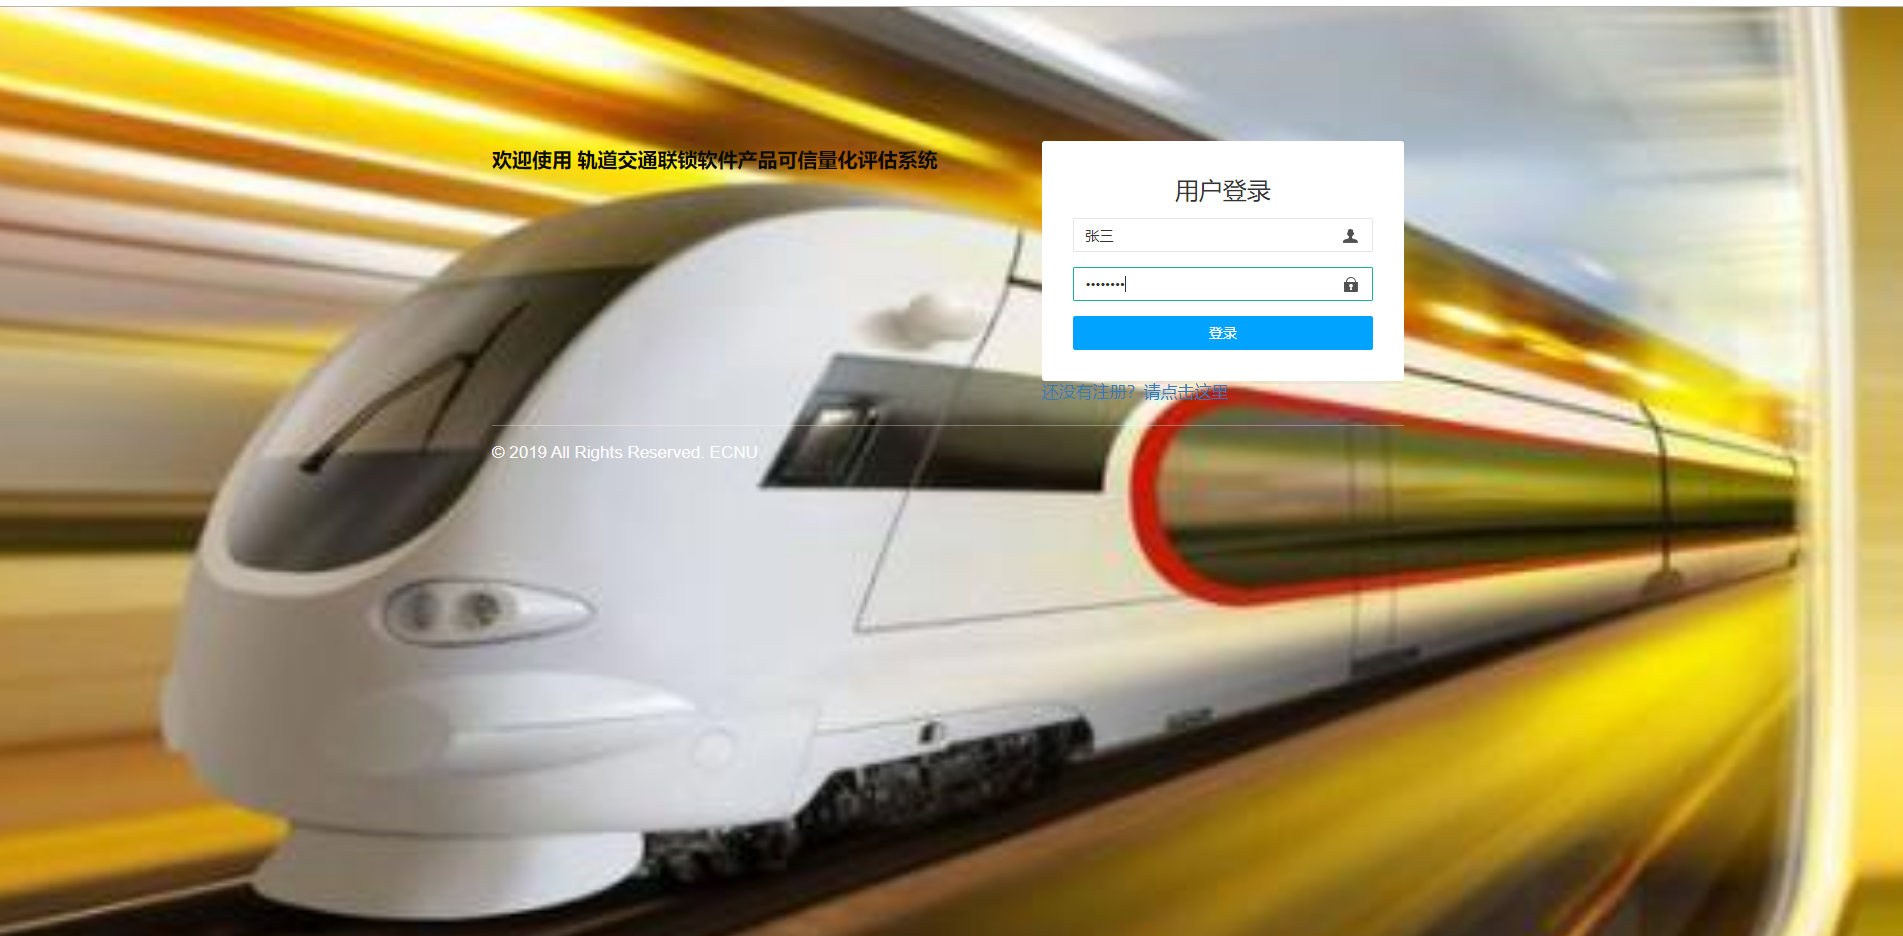
\includegraphics[width=13cm]{fig/5_13.png}
	\caption{登录界面}
	\label{fig:5_14}
\end{figure}



软件产品管理包括产品基本信息维护和人员(用户)信息维护。

(1)软件产品基本信息维护

产品基本信息即产品编号,产品名称,产品状态(待评测、评测结束),项目组长,开发负责人等。点击添加按钮,增加测评软件信息。默认新增的测评软件状态为待评测,可信值为0。操作栏的图标从左至右分别表示编辑、删除、查看报告。点击编辑图标按钮即可对软件信息进行编辑。点击删除图标按钮即可删除软件,此操作会将与该软件有关的所有信息如度量数据、评测数据全部删除。待软件的状态为评测结束之后,点击查看报告图标按钮可查看评测报告,状态为待测评测该按钮是不可用的。
\begin{figure}[htb]
	\centering
	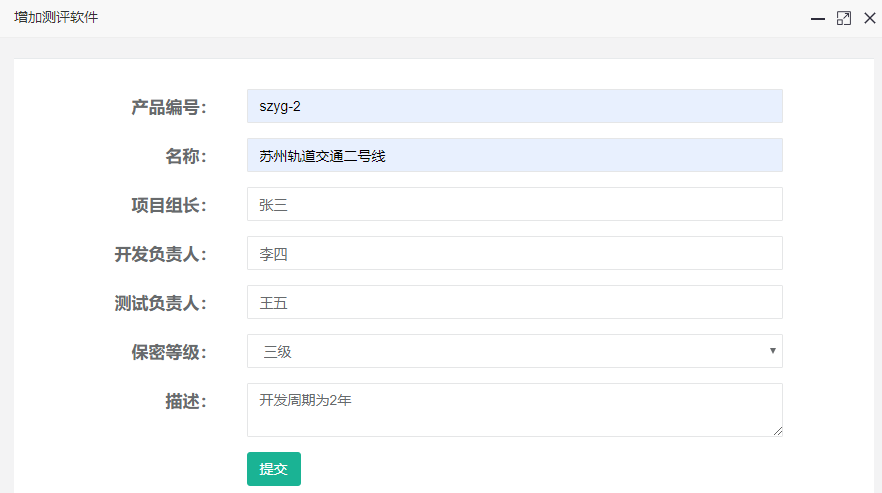
\includegraphics[width=13cm]{fig/sy5_12.png}
	\caption{增加待评估软件}
	\label{fig:5_12}
\end{figure}

\begin{figure}[htb]
	\centering
	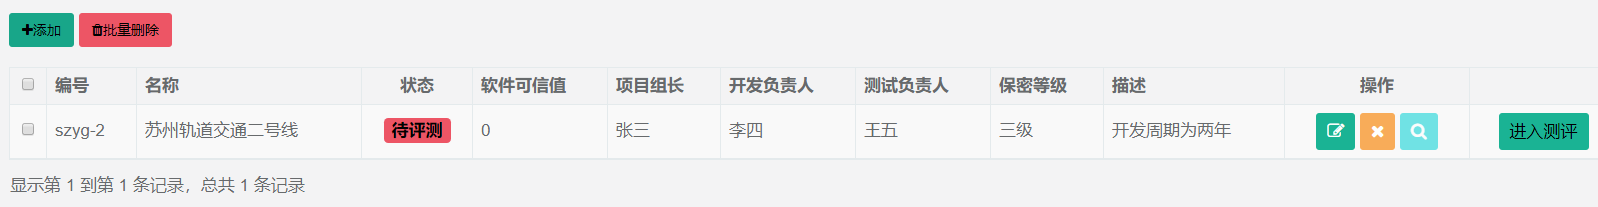
\includegraphics[width=13cm]{fig/sy5_13.png}
	\caption{产品信息维护界面}
	\label{fig:5_13}
\end{figure}

(2)人员信息维护

人员(用户)信息包括姓名,部门,分组,邮箱等。主要是跟待评估软件相关的工作人员。状态分为正常和离职,管理员可删除离职的员工。点击添加按钮,增加工作人员,填写人员基本信息,填写完成点击提交,格式不符合要求的信息会有提示。
\begin{figure}[htb]
	\centering
	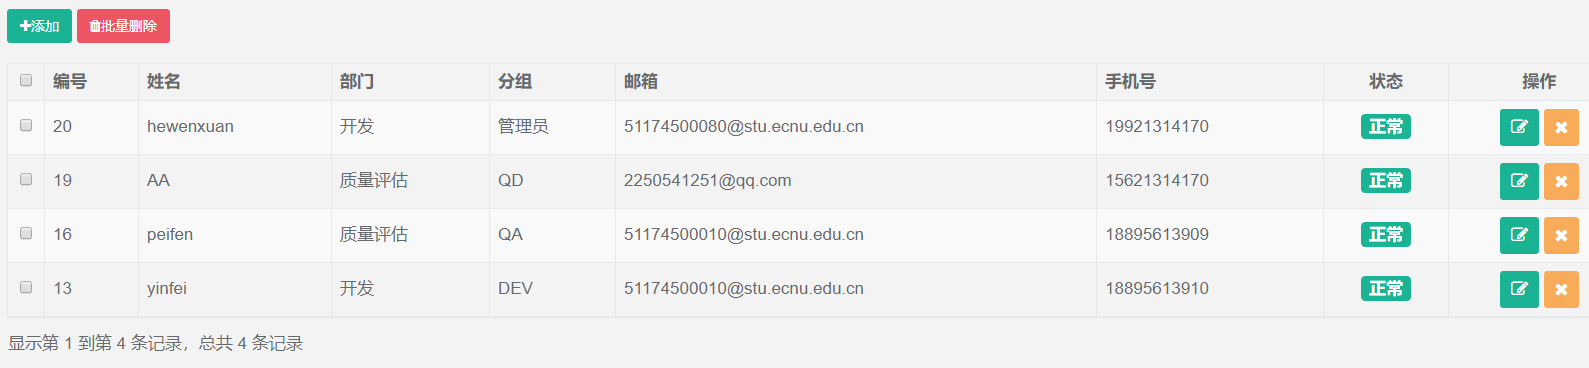
\includegraphics[width=13cm]{fig/5_05.png}
	\caption{人员信息维护界面}
	\label{fig:5_14}
\end{figure}

接下来就是对软件产品开发的四个阶段进行可信评估。需求阶段首先左侧导航栏的可信证据上传,然后点击下载模板的链接,参考模板文件中的格式,本地计算机中填写需求阶段可信证据Excel文件。接着点击选择,弹出文件对话框,选择要上传的文件,点击上传按钮,上传成功或者文件格式不符合要求会弹出提示。打开本地文件之后,点击移除按钮可移除文件,重新选择文件。文件上传成功之后,会自动刷新请求数据库,将当前测评软件的需求阶段可信证据用表格的形式显示。分页功能会显示总共多少条记录,可选择每页显示多少条记录,可选择性查看具体哪一页的记录,并且可以返回首页,跳到尾页。
\begin{figure}[htb]
	\centering
	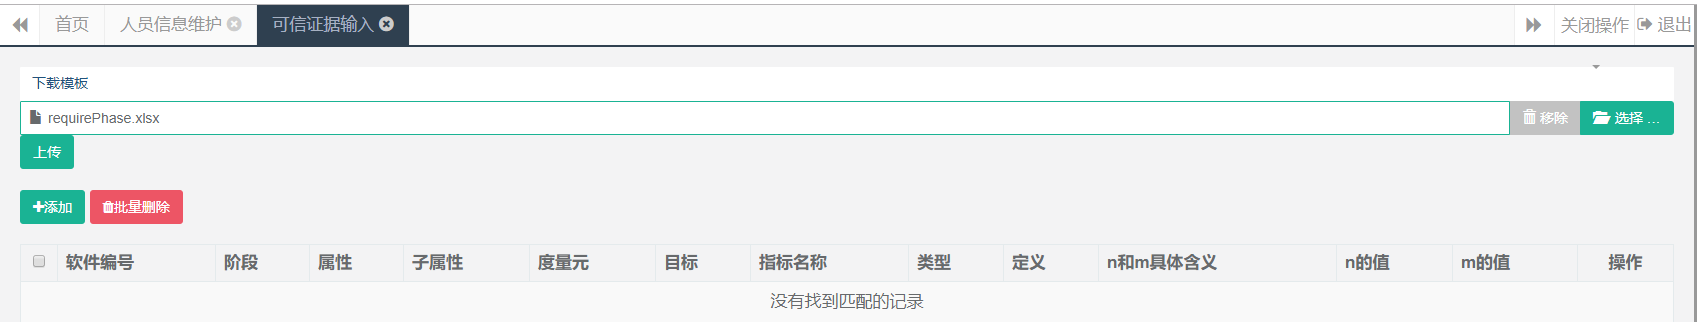
\includegraphics[width=13cm]{fig/sy5_15.png}
	\caption{上传可信证据Excel文件}
	\label{fig:5_15}
\end{figure}

点击添加按钮,增加一条可信证据,填完信息点击提交,或者可点击重置重新填写。选中想要删除的度量数据,点击批量删除按钮,可一次删除多条记录,避免了逐条删除的麻烦。

\begin{figure}[htb]
	\centering
	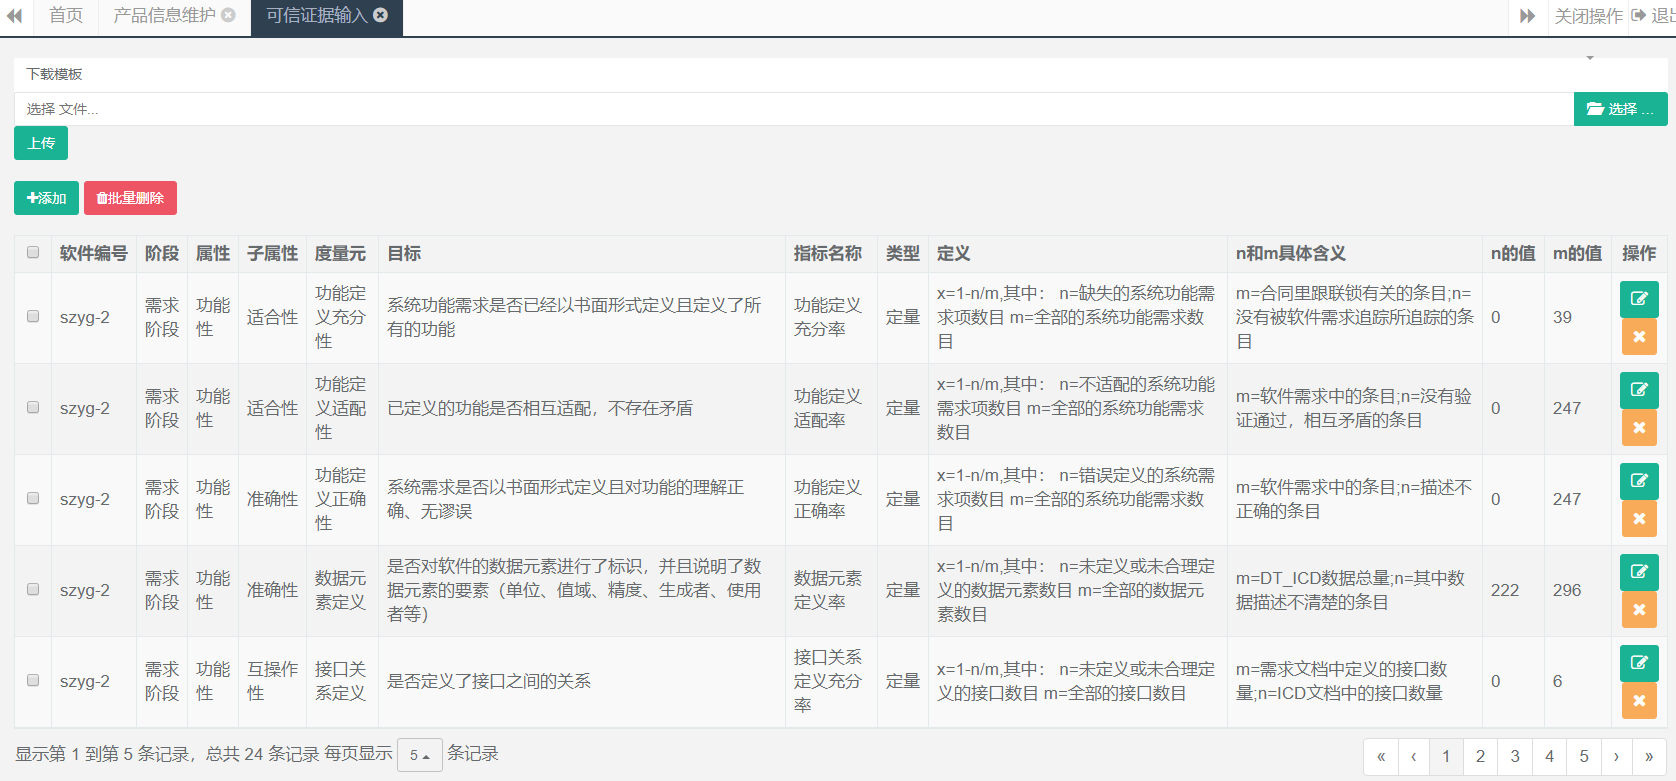
\includegraphics[width=13cm]{fig/sy5_16.png}
	\caption{可信证据上传成功}
	\label{fig:5_16}
\end{figure}

权重分配首先录入属性的正互反判断矩阵,每页都点击下一步直到度量元正互反矩阵录入完毕,点击提交,三个正互反矩阵都通过一致性检验之后,跳转到权重显示页面。
\begin{figure}[htb]
	\centering
	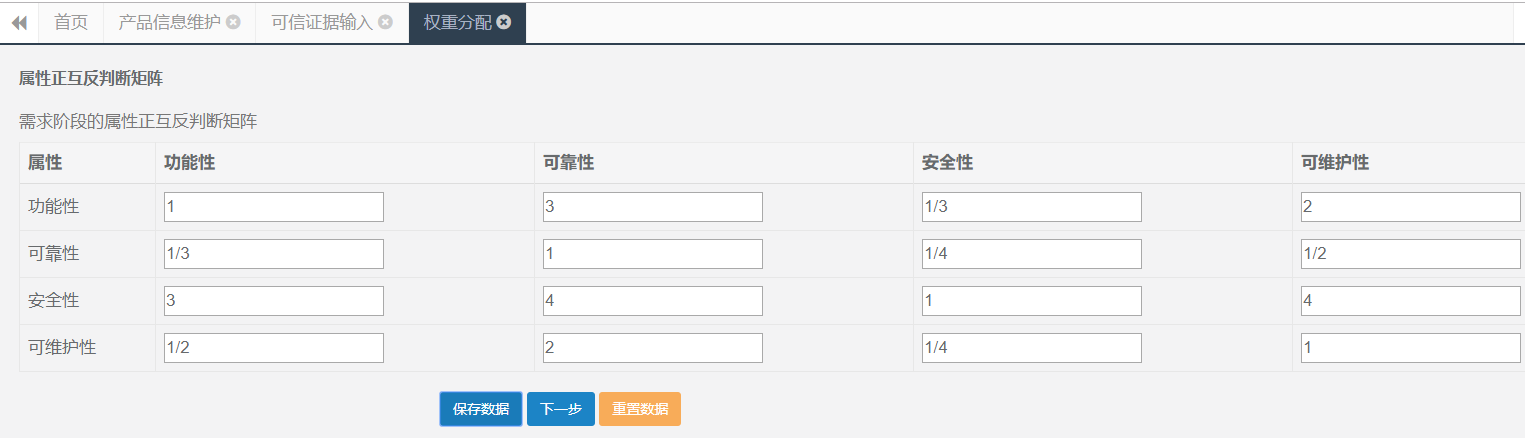
\includegraphics[width=13cm]{fig/sy5_17.png}
	\caption{属性正互反矩阵}
	\label{fig:5_17}
\end{figure}
\begin{figure}[htb]
	\centering
	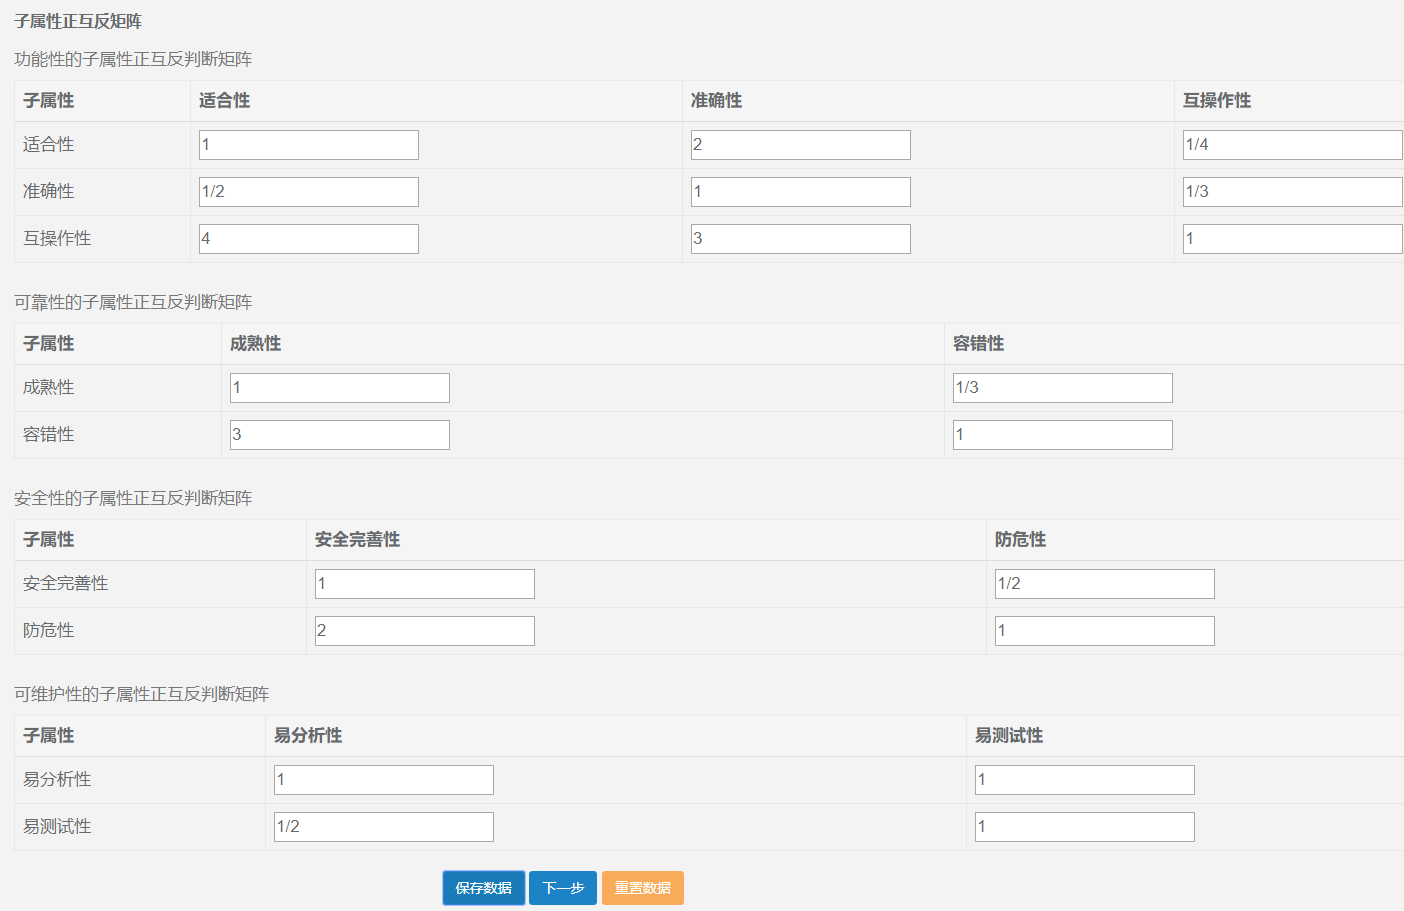
\includegraphics[width=13cm]{fig/sy5_18.png}
	\caption{子属性正互反矩阵}
	\label{fig:5_17}
\end{figure}
\begin{figure}[htb]
	\centering
	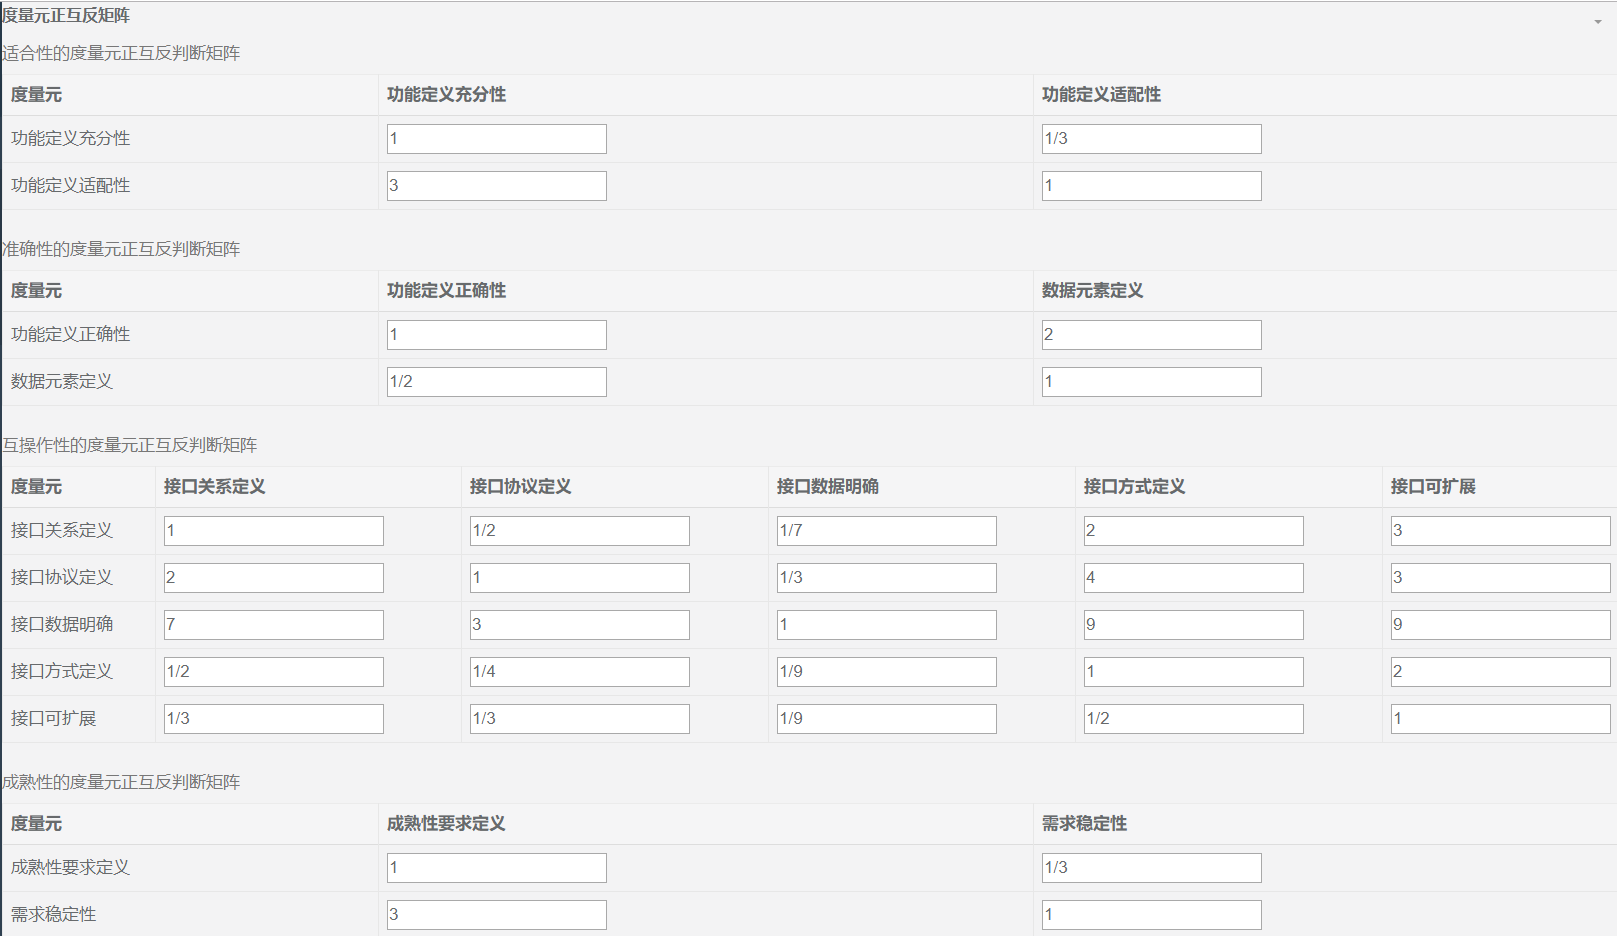
\includegraphics[width=13cm]{fig/sy5_19.png}
	\caption{度量元正互反矩阵}
	\label{fig:5_17}
\end{figure}

\begin{figure}[htb]
	\centering
	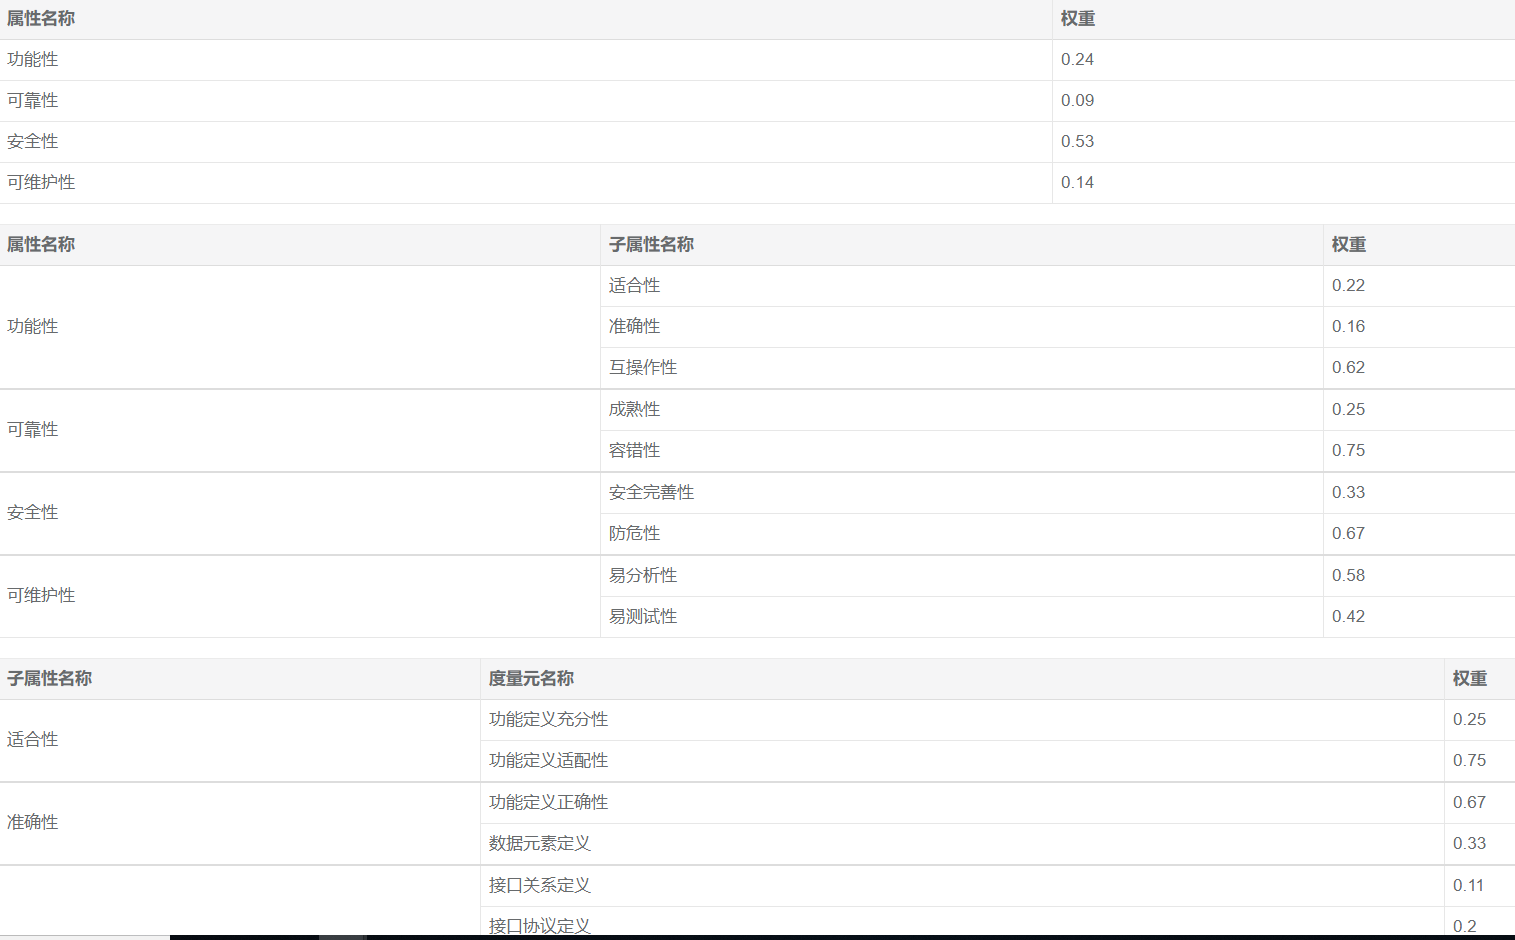
\includegraphics[width=13cm]{fig/sy5_19_1.png}
	\caption{权重显示}
	\label{fig:5_18}
\end{figure}

点击可信值计算按钮,后台根据可信度量模型的公式进行可信值计算,并将计算结果显示在页面上,如图中的需求阶段可信度,每个属性的可信度,每个子属性的可信度。
\begin{figure}[htb]
	\centering
	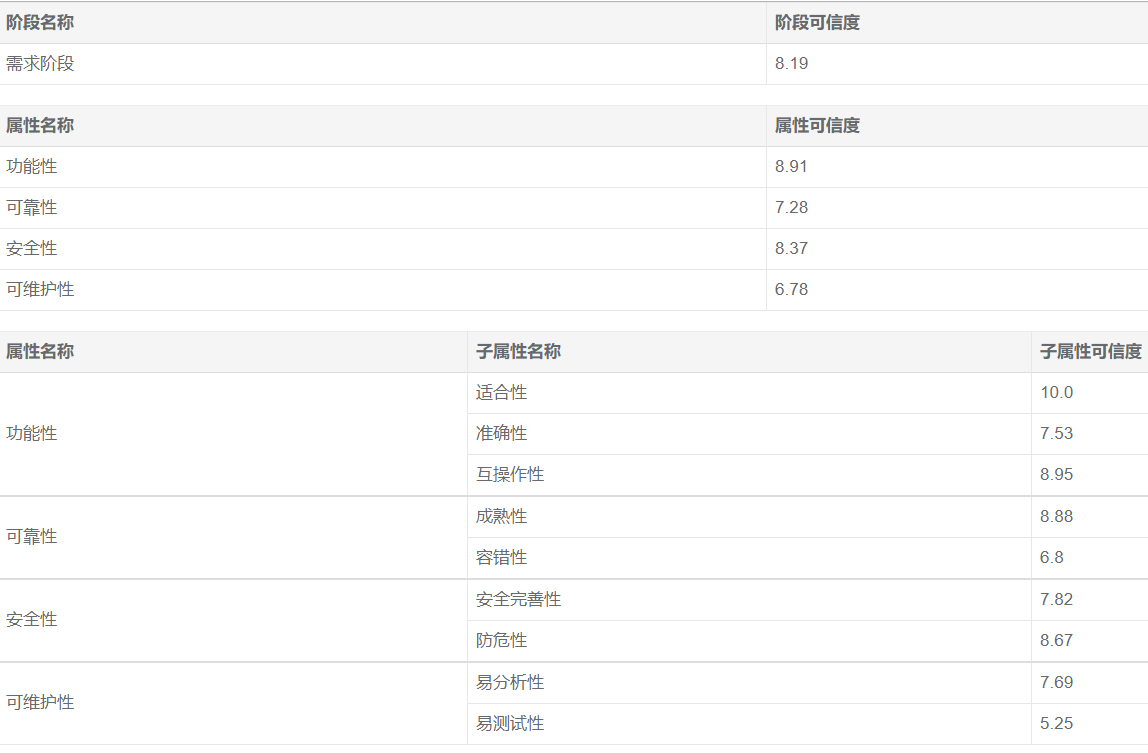
\includegraphics[width=13cm]{fig/sy5_19_2.png}
	\caption{可信值计算结果}
	\label{fig:5_19}
\end{figure}

设计、编码和测试阶段操作同需求阶段。

点击左侧导航栏的数据可视化,查看每个阶段属性子属性可信值图谱和堆叠条形图。如果想查看每个阶段评估的具体信息,点击表格分析。
\begin{figure}[htb]
	\centering
	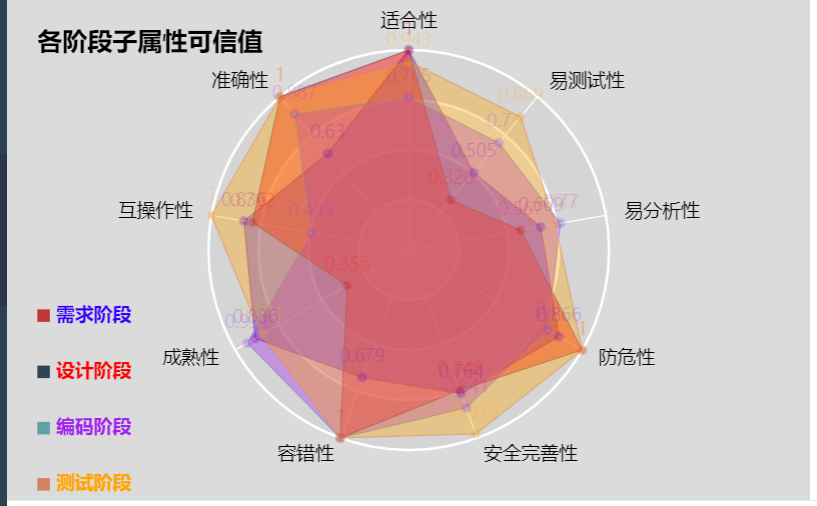
\includegraphics[width=13cm]{fig/sy5_20.png}
	\caption{四个阶段子属性可信值图谱}
	\label{fig:5_20}
\end{figure}

\begin{figure}[htb]
	\centering
	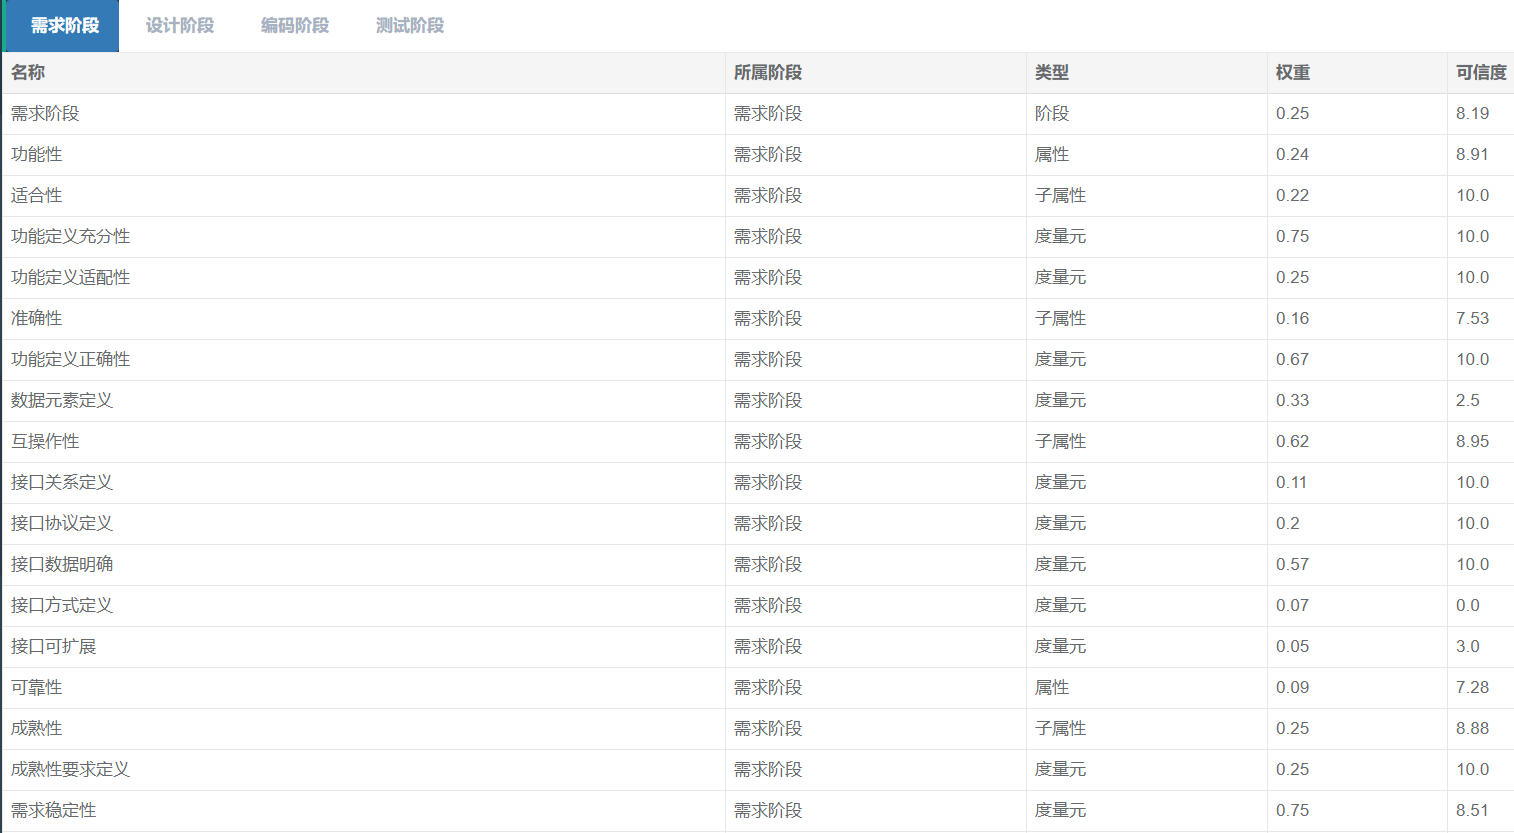
\includegraphics[width=13cm]{fig/sy5_19_4.png}
	\caption{可信值表格分析}
	\label{fig:5_21}
\end{figure}

最后点击生成评估,查看苏州有轨2号线联锁软件的可信评估报告结果。该软件的可信值为8.43,可信等级是\uppercase\expandafter{\romannumeral3},报告中给出了提高可信等级的具体建议,相关决策人员可参考。
\begin{figure}[htb]
	\centering
	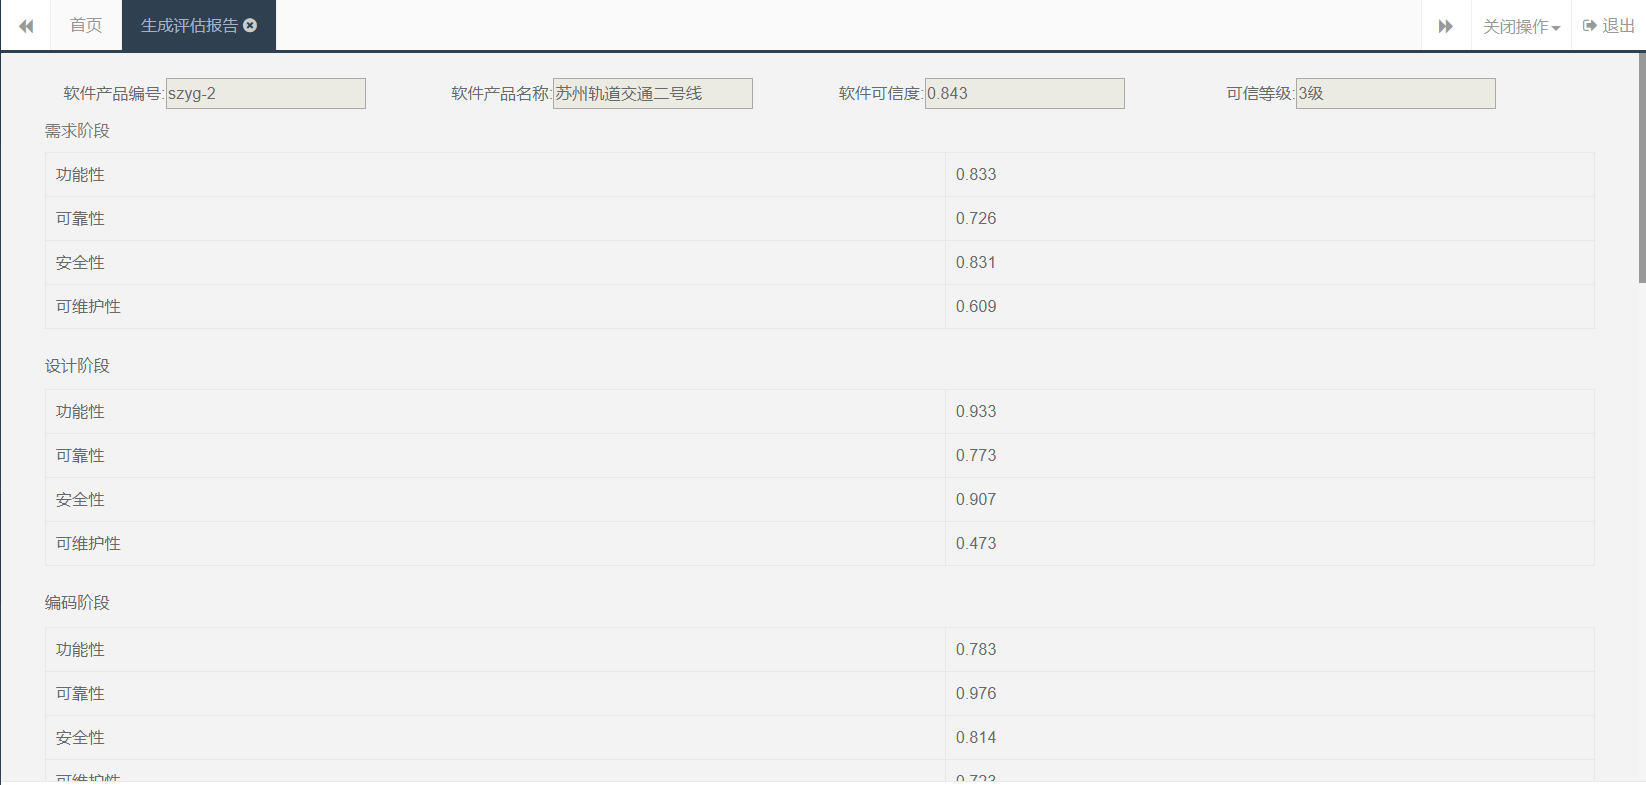
\includegraphics[width=13cm]{fig/sy5_22.png}
	\caption{评估报告}
	\label{fig:5_22}
\end{figure}

此时,刷新页面,点击产品基本信息维护,当前测评软件的状态已从待评测变为评测结束,可信值也给出,点击操作栏的查看报告图表标也可以查看评测报告。
\begin{figure}[htb]
	\centering
	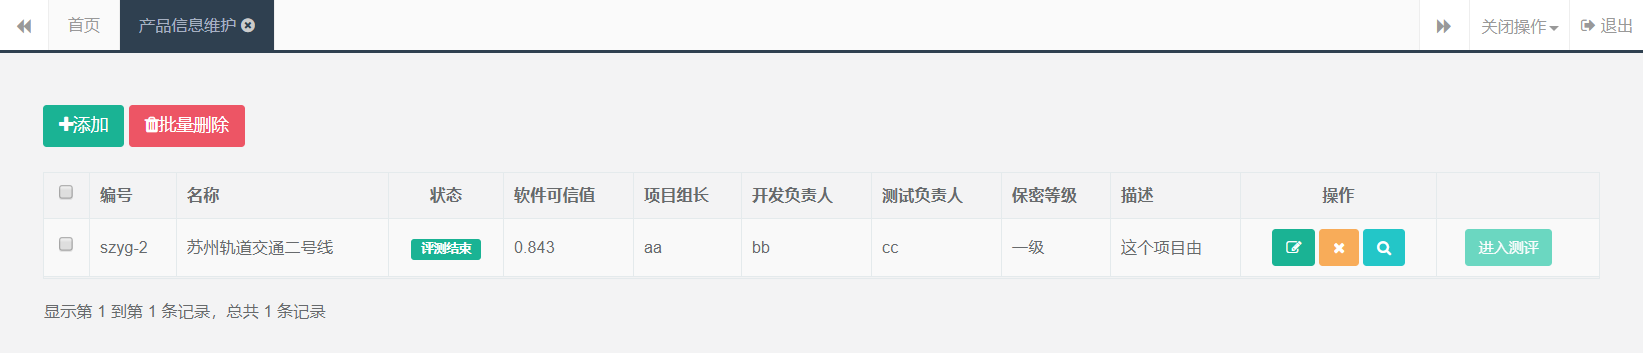
\includegraphics[width=13cm]{fig/sy5_23.png}
	\caption{软件产品评估结束对应的产品信息}
	\label{fig:5_23}
\end{figure}

\section{本章小结}
本章主要介绍了轨道交通联锁软件可信评估工具的分析、设计与实现,并以富欣公司所做的苏州有轨二号线联锁软件为例,阐述了工具使用流程。该工具实现了不同软件基本信息的管理。用户针对不同软件可自定义每个阶段的可信证据表,上传到工具,实现软件全生命周期的可信评估。工具以图表这种非常直观的形式,让用户了解软件每个阶段的可信评估情况。当前软件评估结束之后,根据可信等级,对当前软件以及软件开发过程提出指导建议,并在评估报告中展示。


% \section{系统框架}
 
%  \subsection{架构设计思路}                                                            本系统采用的Web系统开发,前端用于与用户的交互,通过前端请求,传送的数据到后台进行处理,后台使用模型的计算处理算法与相关的业务逻辑处理,在这个过程中,还需要数据库来存储相关的信息,所以需要使用数据库服务器和应用服务器,然后使用开源集成服务器WarmServer在本地离线使用。
%  架构设计原则考虑MVC分层的思想,Model层代表了进行逻辑判断、数据库和XML文件的存取,Controller层代表了中介者的作用,将数据传递给业务逻辑。View层表示了根据业务逻辑选择不同的视图,如图\ref{MVC2}所示。            
 
%  使用语言html5+css3+javascript+php7+mysql+xml。
 
%  前端框架bootstrap,后台mvc模式。
 
%  开发工具:PHPstorm2016.2.1。
 
%  部署工具平台:WampServer(开源集成工具)。
 
%  适用平台:Windows/linux。
 
% %本节进一步介绍Cppcheck工具的界面和内嵌检查类。Cppcheck使用C++语言进行开发,提供了对C/C++多种类型错误的检查,其检查点涉及指针、数组、内存以及函数中的问题。
% %选取Cppcheck作为本工具的研究基础,是因为Cppcheck是开源工具,并且Cppcheck开放了用户扩展接口,使得开发者很容易将自定义的规则嵌入Cppcheck中,
% %定制个性化的检查工具。
% \begin{figure}[htb]
% 	\centering
% 	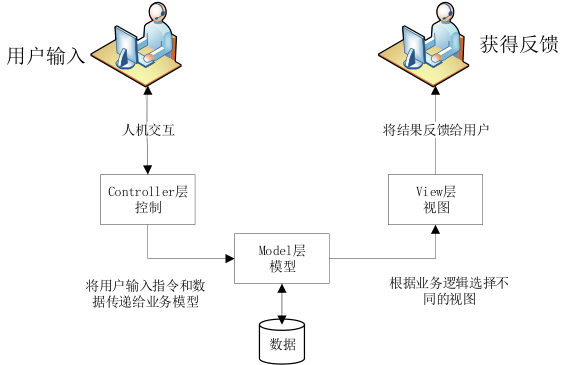
\includegraphics[width=10cm]{fig/MVC2.jpg}
% 	\caption{MVC分层}
% 	\label{MVC2}
% \end{figure}

% \subsection{系统建模}

% 评估软件可信性需要计算需求分析阶段、软件设计阶段、软件编码阶段与软件阶段四个阶段的可信性,每个阶段导入以可信证据指标-度量元-子属性-属性的模板文件,生成可信证据采集页面,每个阶段输入相关的可信证据即可。根据设定的模型算法,计算可信证据指标、度量元、子属性、属性以及每个阶段的可信性,最后计算出软件可信性以及确定软件可信级别。在这个过程需要权重计算功能实现软件度量元、子属性、属性的权重初始分配。如图\ref{require}用例图所示,根据实际使用需求,可以评估不同项目可信性,需要项目管理,功能用于创建项目与输入项目有关信息,数据分析用于显示软件属性等相关信息,评估报告用于输出整个项目整体情况,增加权限管理用于管理人员,实现不同项目小组评估不同的项目等功能。

% \begin{figure}[htb]
% 	\centering
% 	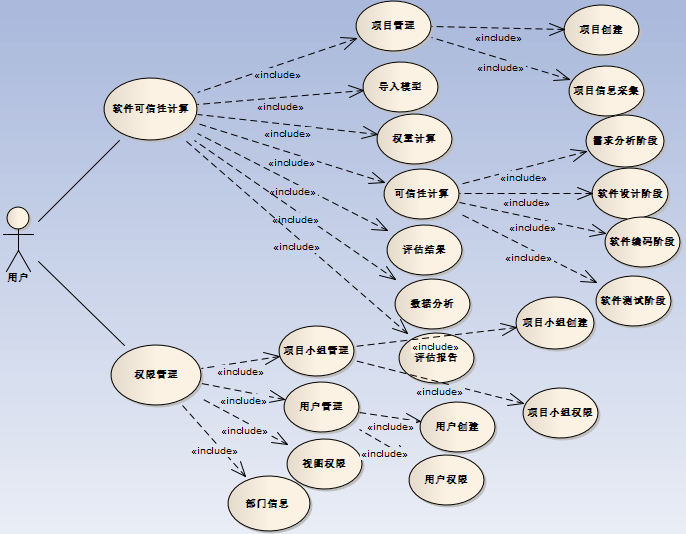
\includegraphics[width=10cm]{fig/require.jpg}
% 	\caption{系统用例图}
% 	\label{require}
% \end{figure}

% \subsection{系统功能}
% 基于可信证据的软件可信性计算系统功能如图\ref{zhuzitu}所示。系统可以划分成两大模块,软件可信性计算与权限管理。软件可信性计算模型包含项目创建、项目信息采集、导入模型、权重计算、四个阶段可信性计算、评估结果、数据分析以及评估报告功能。项目创建功能主要是创建当前计算可信性的项目名称、项目代号、项目类型、待评估软件概述与当前项目访问控制等基本功能。项目信息采集主要是包含文档概述、委托方的名称与联系方式、研制方的名称与联系、引用文档、评估方法说明等基本情况的录入。导入模型功能主要根据不同项目,收集的可信证据有所不同,导入适合该项目的四个阶段的可信度量表模板,模板里面包含了属性、子属性、度量元、可信证据指标的信息。该模板使用XML文件存储,利用XML文件树型逻辑结构的特点,属性结点包含子属性结点,子属性结点包含度量元结点,度量元结点包含可信证据指标结点。权重计算功能主要计算软件属性、子属性权重,计算软件不同阶段可信度量元权重,同时判断计算属性权重、子属性权重、度量元权重是否符合一致性要求。四个阶段可信性计算功能依赖前面导入模型与权重计算,导入模型完毕后,利用XML解析算法与后台算法,在四个阶段生成输入页面。当前面的权重计算符合要求,权重值除了显示在权重计算页面,同时所有计算的权重值保存到XML文件,同时在四个阶段生成页面显示出权重值。因此,四个阶段可信性计算主要功能为可信证据指标采集相应的数据,通过前面设定的可信性计算框架算法计算出结果。评估结果主要功能根据前面四个阶段计算出的可信性值,加权平均得到软件的可信值,通过设定的分级评估算法,确定软件的可信级别。数据分析主要通数据库保存的相应信息,查询项目不同阶段属性或子属性或全部信息或者只查看某一个属性,通过表格显示出每一步的计算结果值。通过饼状图、柱形图与雷达图分析属性或子属性的数据结果。评估报告主要功能依赖于前面
% 项目创建时的基本信息、项目信息采集的基本信息、软件四个阶段的可信值、软件整体的可信值与软件的可信级别、通过表格、柱形图、雷达图、饼状图显示可视化显示相关的信息以及报告输出功能。

% 权限功能主要包括创建用户、用户信息管理、用户权限管理、项目小组创建、基本信息管理、项目小组权限等功能,权限功能主要作用分配相应的项目小组,不同的项目小组负责会在实际操作中负责不同的项目,不同的项目小组人员也会负责不同的项目,所以每个项目在评估软件可信性的时候都会记录哪个小组哪个人员负责处理的该项目的基本信息。项目小组对组内的人员进行不同权限分配,视图权限主要是规定有的用户无法进行权限分配,不能进入权限管理功能。

% \begin{figure}[htb]
% 	\centering
% 	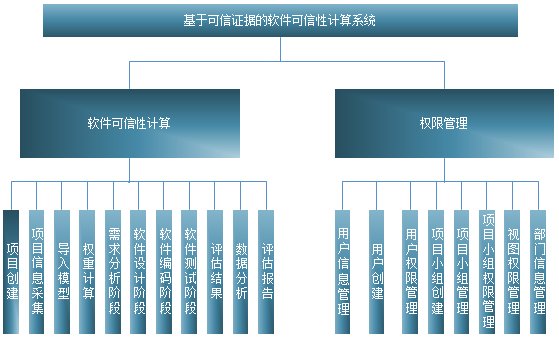
\includegraphics[width=13cm]{fig/zhuzitu.png}
% 	\caption{系统功能模块}
% 	\label{zhuzitu}
% \end{figure}

% \subsection{系统流程}

% 在进行软件可信性计算之前,在权限管理模板确定好评估软件可信性的人员,创建需要评估的软件项目,收集相关的可信证据保存到XML文件中,建立属性-子属性-度量元-可信证据指标的关系。如图\ref{se}为进行软件可信性计算的时序图,输入项目有关信息,进行项目信息采集;导入XML文件,XML文件包含属性、子属性、度量元与可信证据指标基本信息;权重计算依赖于前面模型的导入,因为不同项目的度量元与可信证据指标不同,根据当前项目的度量元进行权重的计算;软件可信性计算包含了从需求分析阶段到软件测试的可信性计算,依赖于模型的导入,生成相关的页面,在页面只需要采集可信证据指标规定的值或定性评分即可。通过获得前面权重值的计算与后台设定的可信性计算算法,计算出软件不同阶段以及软件的可信性值,并且保存相关的数据,可提供给评估结果确定软件可信级别与相关的数据分析。

% \begin{figure}[htb]
% 	\centering
% 	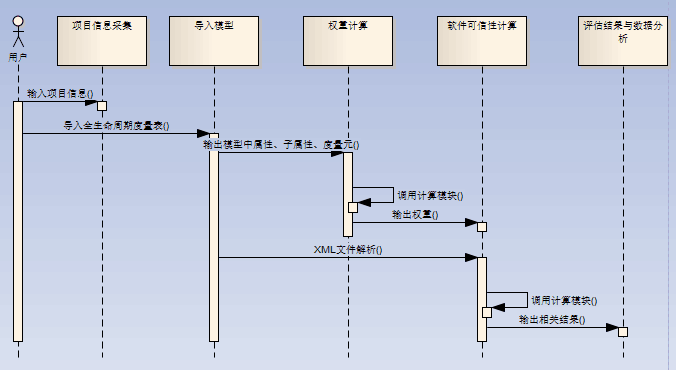
\includegraphics[width=10cm]{fig/se.png}
% 	\caption{软件可信性计算时序图}
% 	\label{se}
% \end{figure}


% \section{工具设计与实现}
% \subsection{界面设计}
% 用户安装软件后,使用浏览器登入系统,用户登录界面如图\ref{login}所示,在用户安装的过程中,第一次会默认设置超级管理员。

%  \begin{figure}[h]
% 	\centering
% 	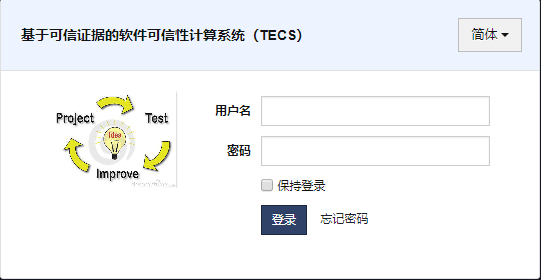
\includegraphics[width=10cm]{fig/login.png}
% 	\caption{登录页面}
% 	\label{login}
% \end{figure}

% 在登录页面输入正确的账号和密码后,系统转到主页面\ref{index}所示,菜单栏分为一级菜单栏与二级菜单栏,一级菜单栏对应主页、软件可信性计算功能和权限管理功能,二级菜单栏为一级菜单栏功能的子功能模块。主页包含登录动态与密码修改功能,登录动态记录所有人员操作的日志信息。

%  \begin{figure}[h]
% 	\centering
% 	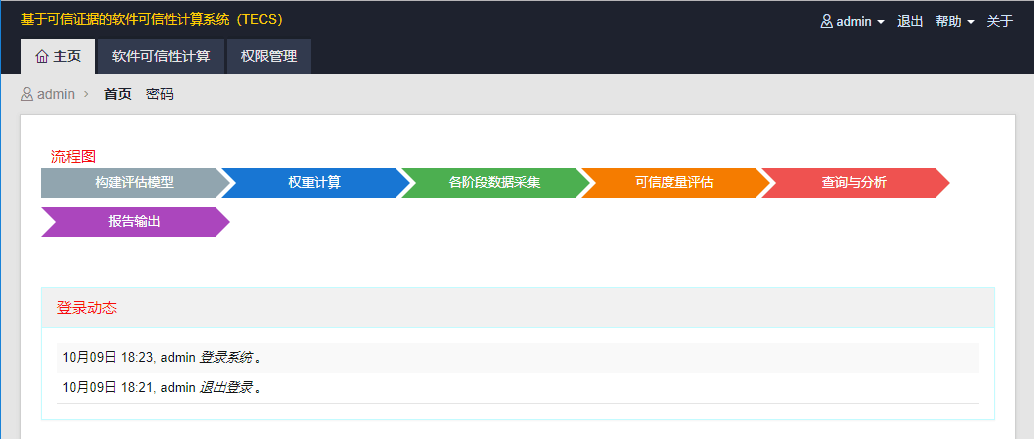
\includegraphics[width=10cm]{fig/index.png}
% 	\caption{主页面}
% 	\label{index}
% \end{figure}

% \subsection{软件可信性计算模块设计}
% 如图\ref{index1}所示,软件可信性计算模块包含了项目创建、编辑项目信息、项目信息采集,导入模型、权重计算、软件需求分析、软件设计、软件编码、软件测试、评估结果、数据分析与评估报告子模块功能。

%  \begin{figure}[htbp]
% 	\centering
% 	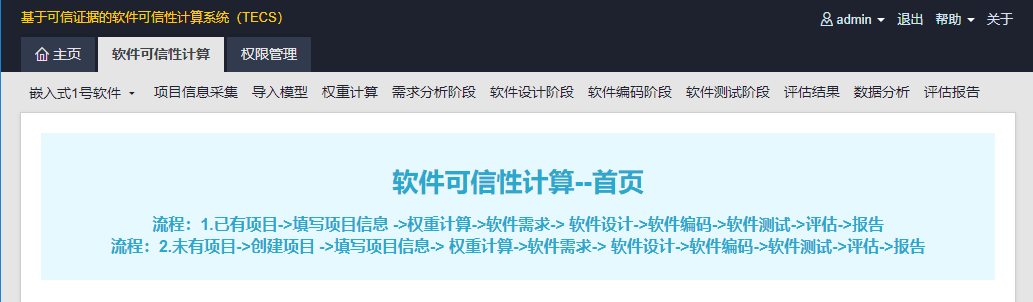
\includegraphics[width=10cm]{fig/index1.png}
% 	\caption{软件可信性计算主页面}
% 	\label{index1}
% \end{figure}

% 评估当前项目软件的软件可信性,首先要创建当前项目的有关信息,如图\ref{create1}所示。
% 输入该项目的名称、代号、项目负责人、项目类型与待评估软件的基本信息概述,确定本项目的权限访问。

%  \begin{figure}[htbp]
% 	\centering
% 	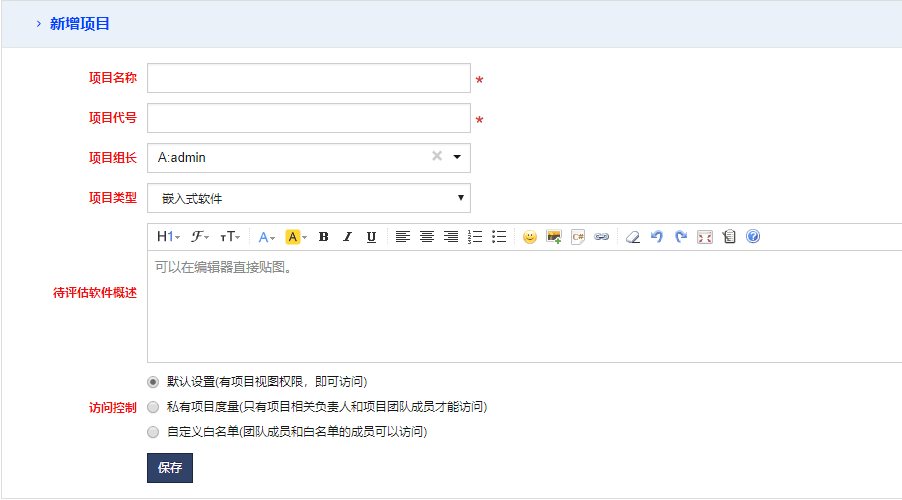
\includegraphics[width=10cm,height=5cm]{fig/create1.png}
% 	\caption{项目创建页面}
% 	\label{create1}
% \end{figure}

% 如图\ref{project1}所示,进行项目信息采集,文档概述、委托方的名称与联系方式、研制方的名称与联系方式、测评机构的名称与联系方式、参考的引用文档、评估方法说明等基本情况,作为后续报告输出的表头部分内容。

%  \begin{figure}[htbp]
% 	\centering
% 	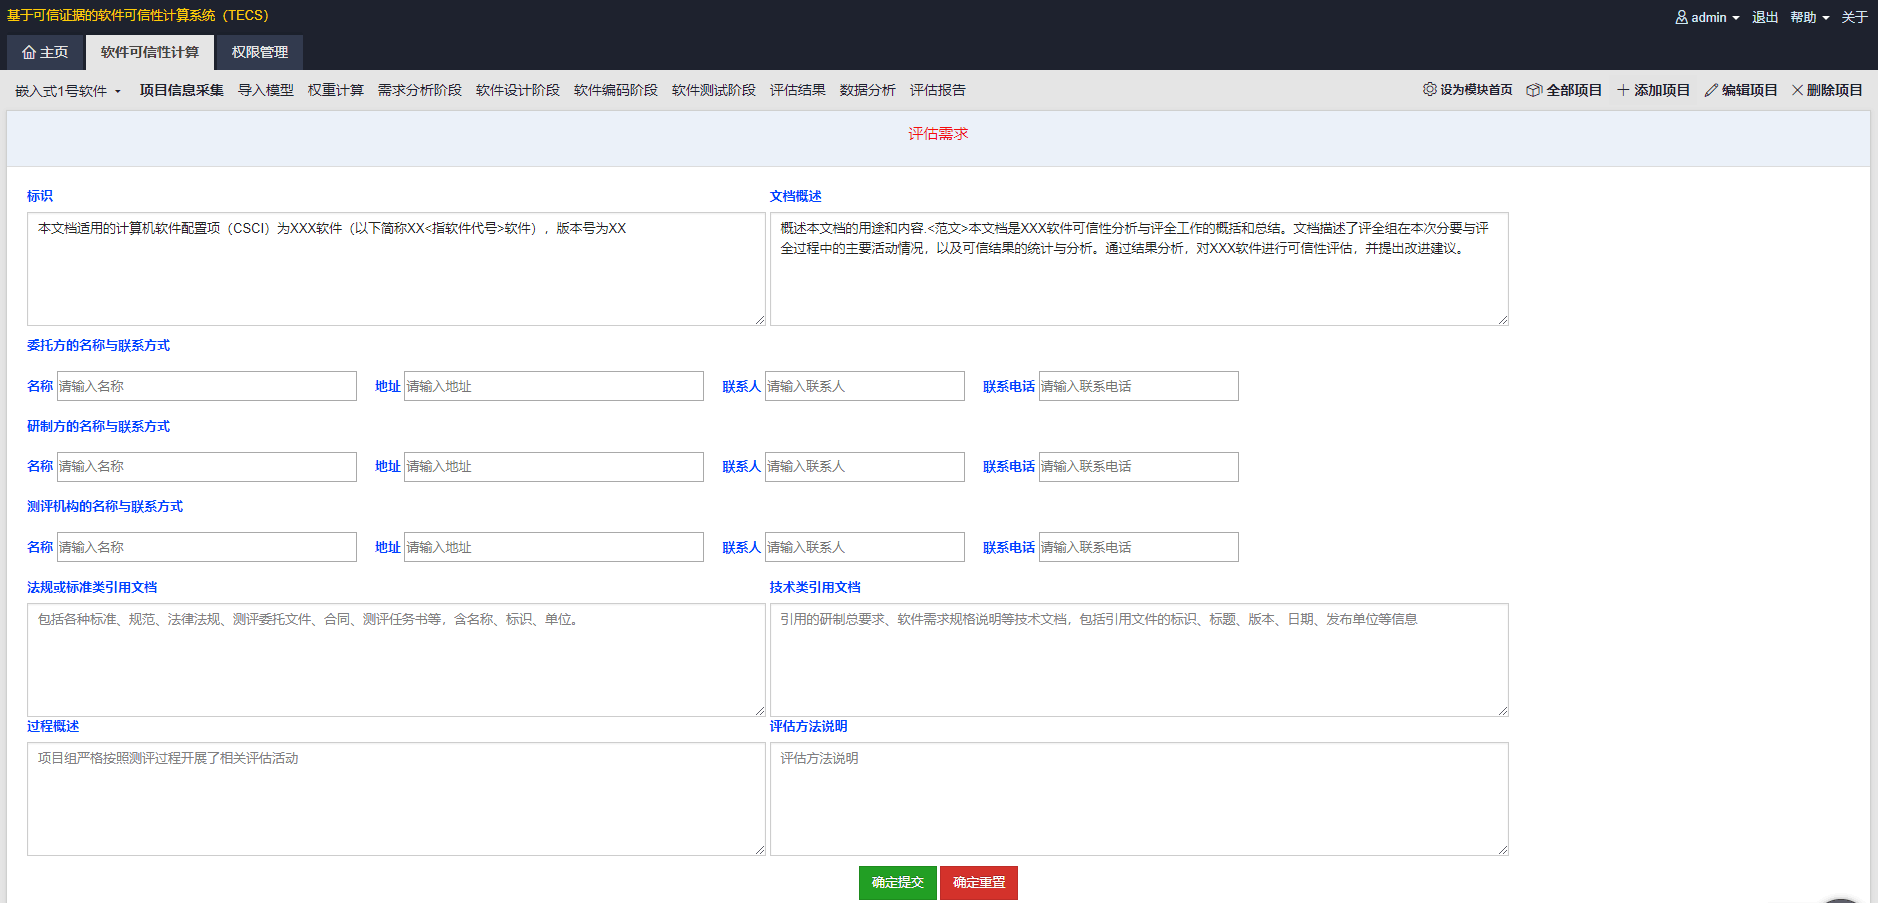
\includegraphics[width=10cm]{fig/project1.png}
% 	\caption{项目信息采集页面}
% 	\label{project1}
% \end{figure}

% 导入模型页面如图\ref{model}所示,从本地文件导入需求分析阶段、软件设计阶段、软件编码阶段以及软件测试阶段XML 模板文件,模板文件包含了本项目属性、子属性、度量元以及可信证据指标相关信息,通过XML解析算法,如算法1所示,通过获取文件根节点,XML文件含有唯一的根节点,根节点含有若干个属性、属性含有若干个子属性、子属性含有若干个度量元、度量元含有若干个可信证据指标,循环输出到指定的页面。在需求分析阶段、软件设计阶段、软件编码阶段以及软件测试阶段生成数据采集页面,为软件可信性计算提供输入页面。

% \begin{algorithm}
% 	\caption{解析XML模板文件.}
% 	\label{}
% 	\begin{algorithmic}[1]
% 		\REQUIRE 不同阶段XML模板文件
% 		\ENSURE 生成各个阶段数据采集页面
% 		\STATE function  parseFile($file$)
% 		\STATE this->load(file) ;~~~~~~\COMMENT{加载文件}  
% 		\STATE Root  =this->getElementsByTagName('root');~~~~~~\COMMENT{获取文件根结点}
% 		\STATE Attribute =Root->item(0)->childNodes;~~~~~~\COMMENT{属性}
% 		\FOR{i =0;i<Attribute->length;i++}
% 		\STATE 输出属性相关信息
% 		\STATE subAttribute =Attribute->childNodes;~~~~~~\COMMENT{子属性}
% 		\FOR{j = 0;j<subAttribute ->length;j++}
% 		\STATE 输出子属性相关信息
% 		\STATE Metric =subAttribute->childNodes;~~~~~~\COMMENT{度量元}
% 		\FOR{k= 0;k< Metric ->length;k++}
% 		\STATE 输出度量元相关信息
% 		\STATE index=Metric->childNodes;~~~~~~\COMMENT{可信证据指标}
% 		\FOR{m= 0;m<  index->length;m++}
% 		\STATE 输出可信证据指标
% 		\ENDFOR 
% 		\ENDFOR
% 		\ENDFOR
% 		\ENDFOR
% 		\STATE end function
% 	\end{algorithmic}
% \end{algorithm}

%  \begin{figure}[htbp]
% 	\centering
% 	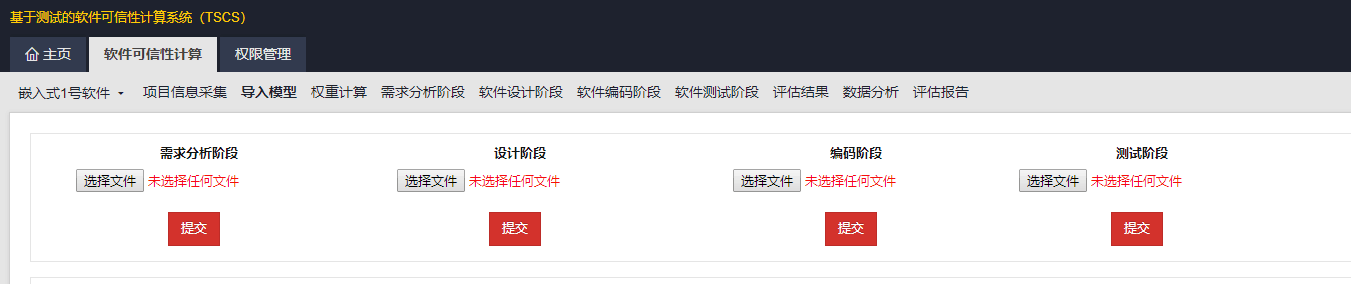
\includegraphics[width=10cm]{fig/model.png}
% 	\caption{导入模型页面}
% 	\label{model}
% \end{figure}


% \begin{algorithm}
% 	\caption{权重计算算法.}
% 	\label{}
% 	\begin{algorithmic}[1]
% 		\REQUIRE 属性或子属性或度量元 判断矩阵 $A$
% 		\ENSURE 属性或子属性或度量元 权重结果 $W$
% 		\STATE function weight($A$)
% 		\STATE N =count(A)~~~~~~\COMMENT{判断矩阵行和列长度}  
% 		\STATE RI =array(0.00, 0.00,0.58, 0.90, 1.12, 1.24, 1.32,1.41, 1.45, 1.51);
% 		\FOR{i=0;i<N;i++}
% 		\STATE w0[i]=bcdiv(1.0,N,17);
% 		\ENDFOR
% 		\STATE delt =0.00001;sum =1.0;d =1.0;
% 		\WHILE{d>delt} % While语句,需要和EndWhile对应
% 		\STATE d=0.0;sum=0;index =0;~~~~~~\COMMENT{获取向量}
% 		\FOR{j =0;j<N;j++}
% 		\FOR{l=0;l<N;l++}
% 		\STATE t+=(A[j][l]*1.0)*w0[l];
% 		\ENDFOR
% 		\STATE w1[j]=t;sum+=w1[j];
% 		\ENDFOR
% 		\FOR{k=0;k<N;k++}
% 		\STATE w2[k]=w1[k]/sum;~~~~~\COMMENT{向量归一化}
% 		\STATE d=max(abs(w2[k]-w0[k]),d); ~~~~~~\COMMENT{最大差值}
% 		\STATE w0[k]=w2[k];~~~~~~\COMMENT{用于下一次迭代使用}
% 		\ENDFOR
% 		\ENDWHILE
% 		\FOR{k=0;k<N;k++}
% 		\STATE lamta+=w1[k]/(N*w0[k]);
% 		\ENDFOR
% 		\STATE CI =(lamta-N)/(N-1);
% 		\IF{CR<0.1}
% 		\STATE 满足一致性检验
% 		\ELSE
% 		\STATE CR>0.1,不满足一致性检验,请重新输入符合条件的正反矩阵
% 		\ENDIF
% 		\RETURN $w2$
% 		\STATE end function
% 	\end{algorithmic}
% \end{algorithm}

% 权重计算页面包含属性权重计算、子属性权重计算和度量元权重,如图\ref{weight}所示,点击属性权重计算功能,显示页面用于输入判断矩阵,方便用户输入,下拉框可选择相应数字。在页面输入判断矩阵,使用算法2进行权重计算。


%  \begin{figure}[htbp]
% 	\centering
% 	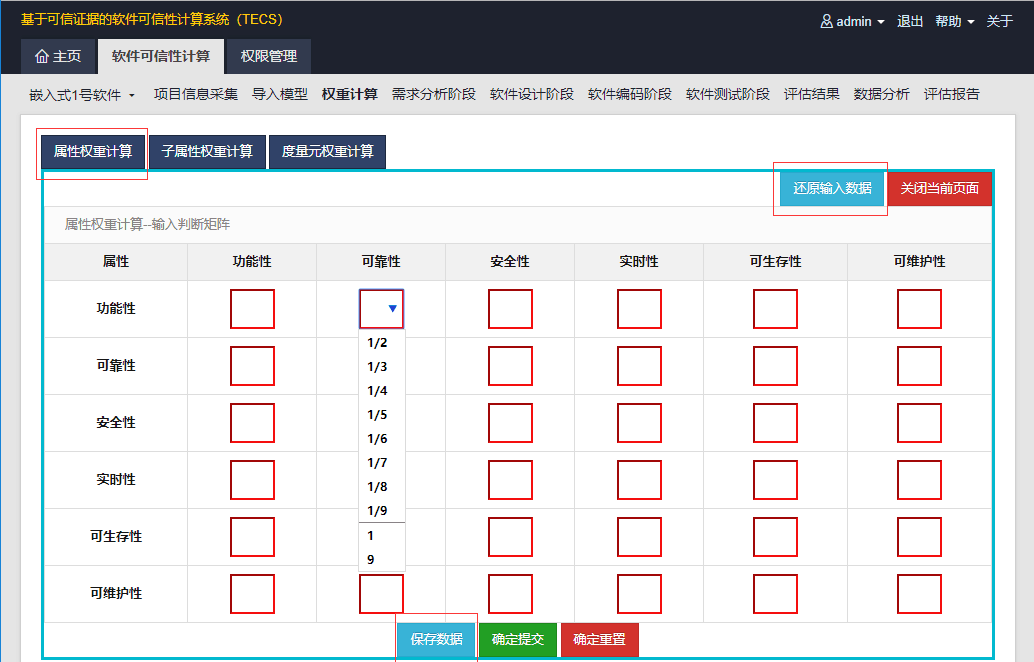
\includegraphics[width=0.6\linewidth]{fig/weight.png}
% 	\caption{属性权重计算页面}
% 	\label{weight}
% \end{figure}

% 本页面为了与用户更好的交互性,使用本地缓存用户输入数据,使用H5的SessionStorage 对象,这些数据不会被保存在服务器上,本地浏览器保存用户的操作,当用户点击保存后,即使遇到浏览器意外关闭等其他情况。重新打开浏览器后,点击还原数据,仍可以还原上一次用户输入情况。点击子属性按钮,权重计算子属性页面如图\ref{subweight}所示,每个属性的子属性都将显示,输入子属性间的判断矩阵,点击提交即可计算出每个属性下面的子属性的权重。

% % \begin{figure}[htbp]
% %	\centering
% %	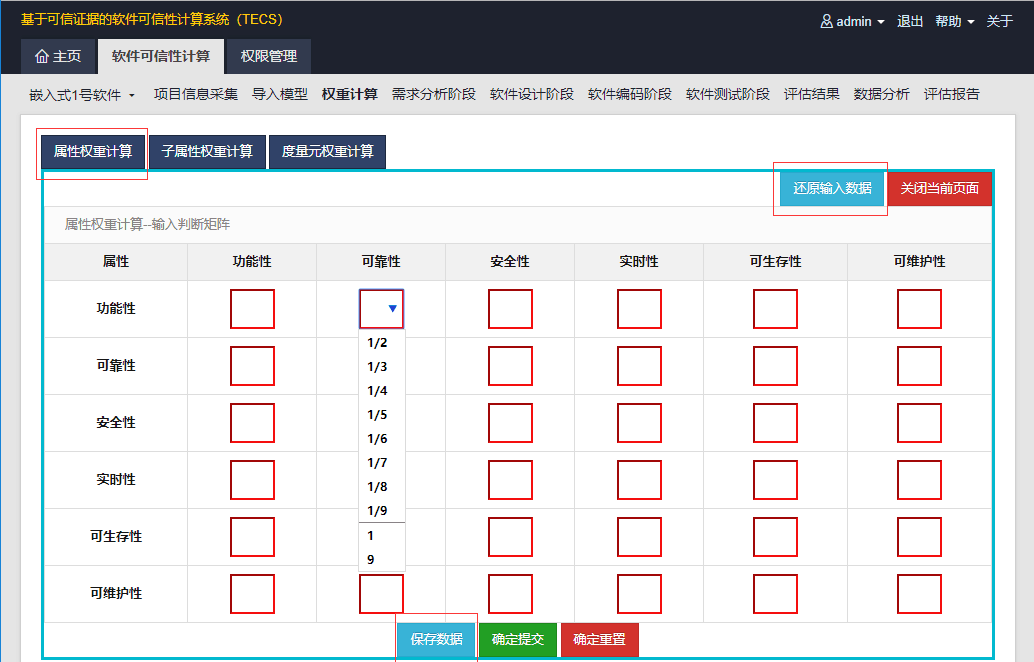
\includegraphics[width=0.6\linewidth]{fig/weight.png}
% %	\caption{属性权重计算页面}
% %	\label{weight}
% %\end{figure}

% \begin{figure}[htbp]
% 	\centering
% 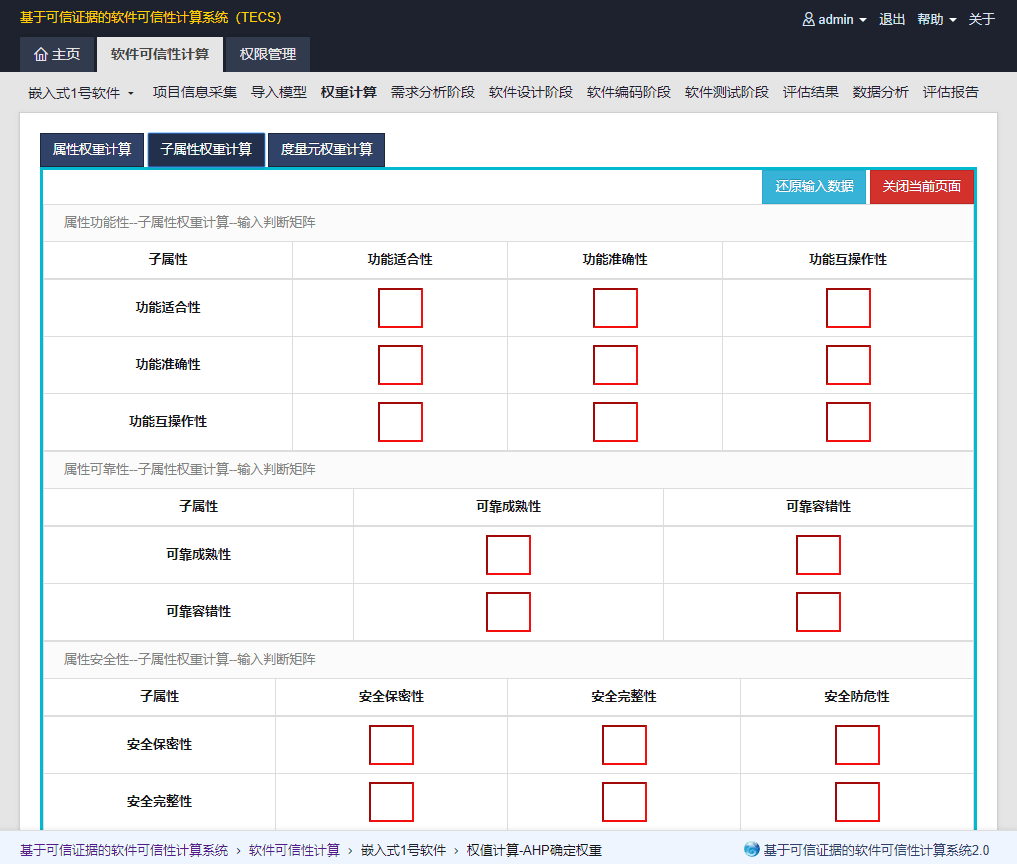
\includegraphics[width=0.6\linewidth,height=6.2cm]{fig/subweight.png}
% 	\caption{子属性权重计算页面}
% 	\label{subweight}
% \end{figure}

% 如图\ref{subsubweight}所示度量元权重计算分为四个阶段,软件需求阶段、软件设计阶段、软件编码阶段于软件测试阶段分别进行权重计算,同理输入正反矩阵。

%  \begin{figure}[h]
% 	\centering
% 	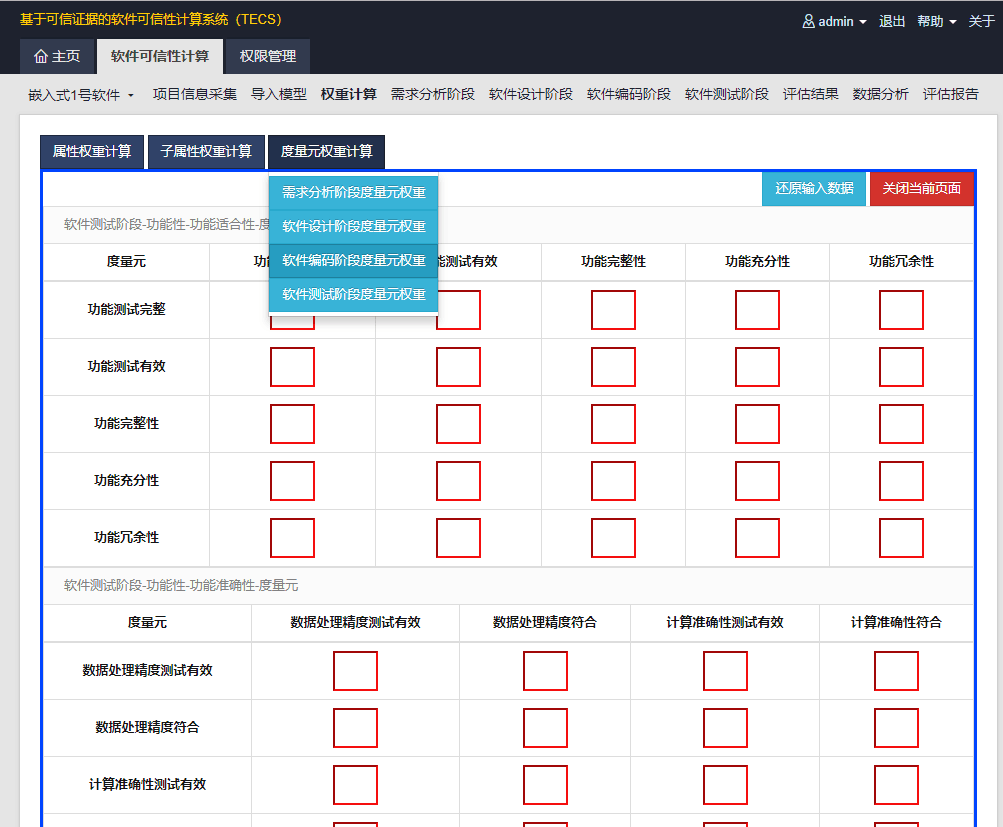
\includegraphics[width=10cm]{fig/subsubweight.png}
% 	\caption{度量元权重计算页面}
% 	\label{subsubweight}
% \end{figure}




% 需求分析阶段、软件设计阶段、软件编码阶段、软件测试阶段依赖于模型的导入,根据不同的项目生成不同的数据采集页面。如图\ref{pingu}所示,当还未进行软件可信性计算,评估结果不会显示任何结果,等待前面可信计算的结果。

%  \begin{figure}[htbp]
% 	\centering
% 	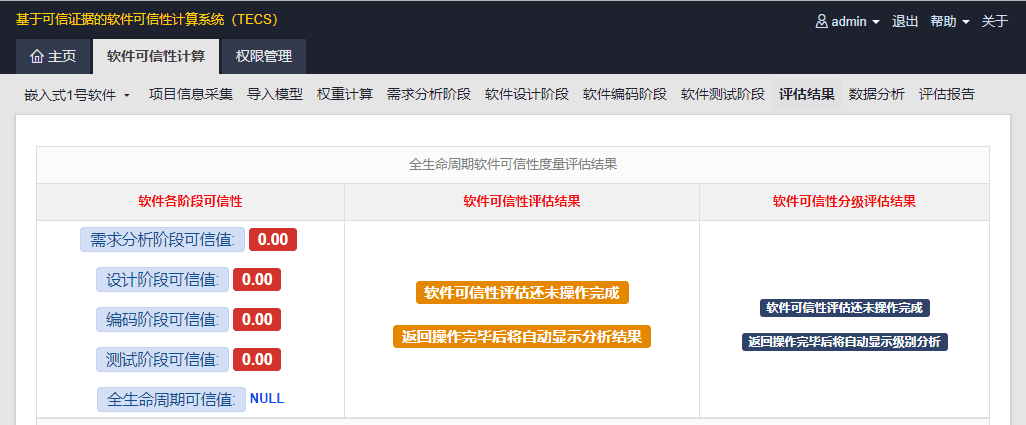
\includegraphics[width=10cm]{fig/pingu.png}
% 	\caption{评估页面}
% 	\label{pingu}
% \end{figure}

% 如图\ref{data1}数据分析页面包含不同阶段,显示属性或子属性或全部信息,也可以单独选取一个属性进行可视化分析,图形主要包含表格图、柱状图、柱形图与雷达图。

%  \begin{figure}[htbp]
% 	\centering
% 	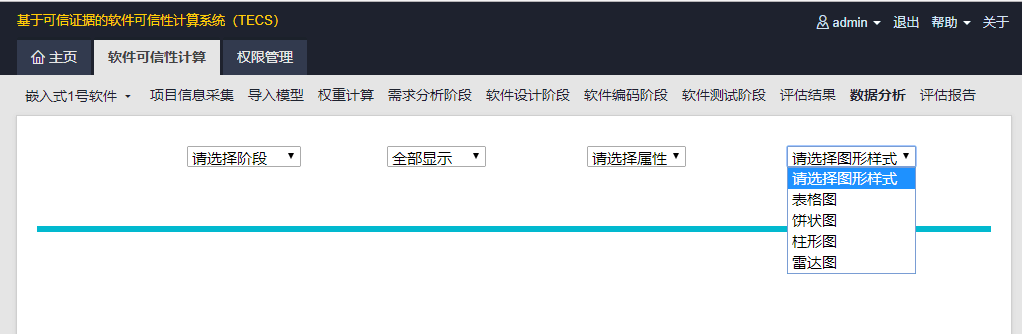
\includegraphics[width=10cm]{fig/data1.png}
% 	\caption{数据分析}
% 	\label{data1}
% \end{figure}

% \subsection{权限管理设计}
% 本节主要是权限管理,包含添加用户或批量添加用户,创建项目组,在项目组分配相应的人员,之后确定该小组的权限与人员可以访问的权限,管理用户基本信息与部门信息管理。如图\ref{quanxian1}所示。

%  \begin{figure}[htbp]
% 	\centering
% 	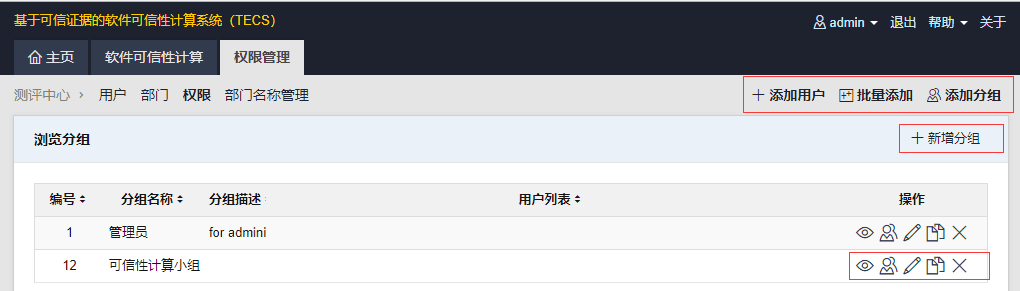
\includegraphics[width=10cm]{fig/quanxian1.png}
% 	\caption{权限管理主页面}
% 	\label{quanxian1}
% \end{figure}

% \section{工具使用}
% 本节模拟工具的使用流程,首先创建一个项目小组,如图\ref{group}所示,建立项目小组名称为测试小组,并在输入框中描述该小组的基本信息。

%  \begin{figure}[htbp]
% 	\centering
% 	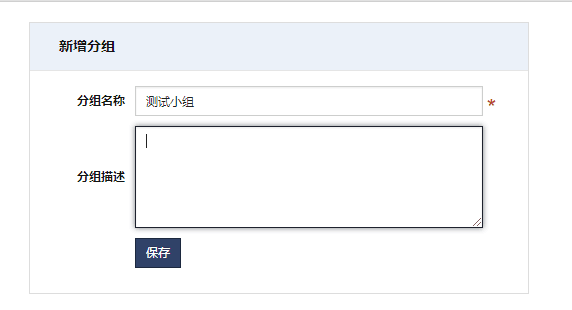
\includegraphics[width=10cm,height=4.6cm]{fig/group.png}
% 	\caption{创建项目小组}
% 	\label{group}
% \end{figure}

% 如图\ref{QA}所示,添加用户基本信息,并且把该用户分配到相应的项目小组。

%  \begin{figure}[htbp]
% 	\centering
% 	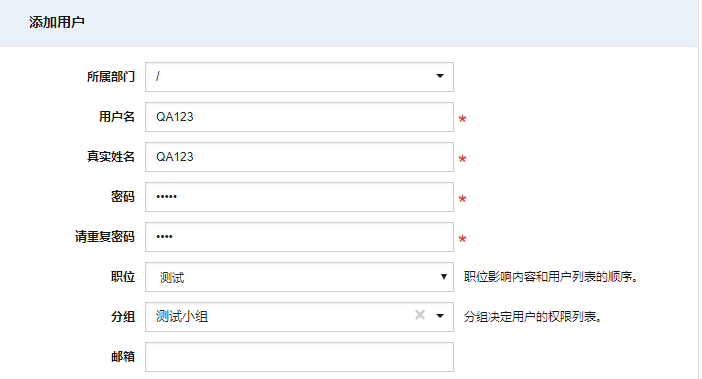
\includegraphics[width=10cm]{fig/QA.png}
% 	\caption{添加用户}
% 	\label{QA}
	
% \end{figure}

% 如图\ref{QA1}通过项目小组人员维护管理,在不添加新的用户的情况下,可以添加其他组的人员参与本项目。

% \begin{figure}[htbp]
% 	\centering
% 	\includegraphics[width=10cm]{fig/QA1.png}
% 	\caption{成员维护}
% 	\label{QA1}
% \end{figure}

% 如图\ref{QA2}所示,设置好该项目小组可以访问视图的权限。

%  \begin{figure}[htbp]
% 	\centering
% 	\includegraphics[width=10cm,height=4.6cm]{fig/QA2.png}
% 	\caption{视图维护}
% 	\label{QA2}
% \end{figure}

% 在前面的基础上,如图\ref{QA3}所示创建需要评估的项目,输入项目名称、项目代号与负责人、项目类型与待评估软件概述信息。在访问控制三种选择,第一种是默认的权限,第二种是规定只有本项目小组的有关人员才能访问此项目,其他项目小组在进行软件可信性评估操作过程中,对该组的项目进行访问没有权限。点击保存,相关信息将录入相关数据库中。

%  \begin{figure}[htbp]
% 	\centering
% 	\includegraphics[width=10cm]{fig/QA3.png}
% 	\caption{创建评估项目}
% 	\label{QA3}
% \end{figure}

% 在项目信息采集页面,输入该项目有关的文档信息,导入模型后,进入权重计算流程。如图\ref{QA4}所示,根据前面属性间重要性,我们可以输入判断矩阵,如果判断矩阵满足一致性。如图\ref{QA5}所示,将输出正确结果,权重值将会自动保存到XML模板文件中。若该矩阵不满足一致性,如图\ref{QA6}所示,输入错误提示结果,结果值不讲保存到XML文件中。同理子属性权重与度量元权重计算相同。

%  \begin{figure}[htbp]
% 	\centering
% 	\includegraphics[width=10cm]{fig/QA4.png}
% 	\caption{属性权重输入}
% 	\label{QA4}
% \end{figure}

%  \begin{figure}[htbp]
% 	\centering
% 	\includegraphics[width=10cm]{fig/QA5.png}
% 	\caption{属性权重结果}
% 	\label{QA5}
% \end{figure}

%  \begin{figure}[htbp]
% 	\centering
% 	\includegraphics[width=10cm]{fig/QA6.png}
% 	\caption{错误提示}
% 	\label{QA6}
% \end{figure}

% 在完成前面流程的基础上,从需求分析阶段,开始可信证据采集,如图\ref{QA7}需求分析阶段所示,只需要输入相关的可信证据数,后台算法自动进行计算,得出度量元的结果值、子属性的结果值、属性的结果值与该阶段的可信性值。同理,软件设计阶段、软件编码阶段与软件测试阶段操作步骤一样。

%  \begin{figure}[htbp]
% 	\centering
% 	\includegraphics[width=10cm]{fig/QS.png}
% 	\caption{需求分析阶段可信证据录入}
% 	\label{QA7}
% \end{figure}

% 在完成前面四个阶段的可信证据采集的基础上,通过前面模型的计算方法与后台的数据处理,在评估结果页面中
% 如图\ref{QA8}所示,将显示该项目不同阶段的可信性值与软件的可信值,并显示该软件的软件可信性级别。

%  \begin{figure}[htbp]
% 	\centering
% 	\includegraphics[width=10cm,height=3cm]{fig/QA8.png}
% 	\caption{软件可信评估结果}
% 	\label{QA8}
% \end{figure}

% 在数据分析页面,如图所示\ref{dataIndex},可选择需求分析、软件设计、软件编码以及软件测试阶段,查看全部信息、属性信息以及子属性信息,也可以选择查看某一个属性的具体信息,可以选择表格图、柱形图、饼图以及雷达图显示。

%  \begin{figure}[htbp]
% 	\centering
% 	\includegraphics[width=10cm]{fig/dataIndex.png}
% 	\caption{数据分析主页}
% 	\label{dataIndex}
% \end{figure}

% 如查看软件测试阶段各个属性的计算结果,如图所示\ref{table.attr}。

%  \begin{figure}[htbp]
% 	\centering
% 	\includegraphics[natwidth=10cm]{fig/table.attr.png}
% 	\caption{各个属性结果值}
% 	\label{table.attr}
% \end{figure}

% 若查看单个属性的全部信息,如图所示\ref{table.single},查看软件测试阶段-属性安全性有关信息。
%  \begin{figure}[htbp]
% 	\centering
% 	\includegraphics[natwidth=10cm]{fig/table.single.png}
% 	\caption{属性安全性}
% 	\label{table.single}
% \end{figure}

% 通过柱形图可视化显示不同属性的结果值,如图\ref{require.drawBarChart}所示。
% \begin{figure}[htbp]
% 	\centering
% 	\includegraphics[natwidth=10cm]{fig/require.drawBarChart.png}
% 	\caption{柱形图显示属性结果值}
% 	\label{require.drawBarChart}
% \end{figure}

% 通过饼状图分析各个属性所占的比例,如图\ref{example1.draw3DPie}所示。

% \begin{figure}[htbp]
% 	\centering
% 	\includegraphics[natwidth=10cm]{fig/example1.draw3DPie.png}
% 	\caption{饼状图显示各个属性占有比}
% 	\label{example1.draw3DPie}
% \end{figure}

% 通过雷达图参看属性值是否均匀分布,如图所示\ref{require.radar.values},

% \begin{figure}[htbp]
% 	\centering
% 	\includegraphics[natwidth=10cm]{fig/require.radar.values.png}
% 	\caption{雷达图显示各个属性分布情况}
% 	\label{require.radar.values}
% \end{figure}

% 最后选择评估报告,本页面将输出所有该项目的所有情况,如图所示\ref{report}。

% \begin{figure}[htbp]
% 	\centering
% 	\includegraphics[width=10cm,height=6cm]{fig/report.png}
% 	\caption{报告输出页面}
% 	\label{report}
% \end{figure}

% \section{本章小结}

% 本章基于前面软件可信性计算模型上,设计完成了基于证据的软件可信性计算系统,该工具实现了不同项目可信证据模型导入、软件不同层次的权重计算、软件需求分析阶段到软件测试阶段的可信性计算,实现了对该软件项目的可信性分级评估。该工具为了满足实际的应用,实现了权限管理系统,使其能根据实际的情况对测试人员及小组进行管理。该工具实现了图形可视化操作,通过数据分析页面,展示不同阶段全部信息或不同属性或不同子属性图形显示操作。该工具实现了本文提出的软件可信性计算模型,完善了基于可信证据的软件可信性计算体系。

